\chapter{Búsqueda de SUSY con fotones y Higgs en el estado final con producción fuerte}
% \addcontentsline{toc}{chapter}{Búsqueda de SUSY con fotones y Higgs en el estado final}
\chaptermark{Búsqueda de SUSY con fotones y Higgs en el estado final con producción fuerte}


% / Tesis lic / %
% El análisis para el cual está orientada esta Tesis consiste en la búsqueda de Supersimetría en eventos con un fotón aislado muy energético, jets y gran cantidad de energía faltante en estado final \cite{Alonso:2147473,ATLAS:2016fks,Collaboration:2198651}. La estrategia general de la búsqueda consiste en el conteo del número de eventos observado en exceso sobre el SM en una cierta región del espacio de observables rica en eventos de la señal considerada.


El trabajo realizado en esta Tesis se centra en la búsqueda de Supersimetría en eventos con un fotón energético y aislado, jets y gran cantidad de energía faltante en el estado final. La estrategia general de la búsqueda consiste en el conteo del número de eventos observado en exceso sobre el SM en una cierta región del espacio de observables rica en eventos de la señal considerada, siguiendo método descripto en el Capítulo \ref{cap:statistical}. El objetivo es poder discriminar de los datos observados aquellos que podrían ser producto de un proceso supersimétricos (señal) de aquellos producto de procesos del SM (fondo).


\section{Muestras de señal a partir de simulaciones de Monte Carlo}

El modelo supersimétrico que motiva a la presente búsqueda consiste en un modelo GGM, por lo tanto la LSP es el gravitino cuya masa será del orden de unos pocos eV. La NLSP es en este caso el neutralino más liviano, que va a consistir en un estado de gauge mezcla de bino y higgsino
% , lo que le permite acoplar a fotones y bosones de higgs
. En particular para esta Tesis se estudia el caso fenomenológico en el cual el neutralino más liviano decae en proporciones iguales a $\gamma+\gravino$ y a $h+\gravino$. Esto último es posible si se elige al parámetro $\mu<0$ que favorece el decaimiento al higgs, y reduce el decaimiento al bosón $Z$, en cuyo caso ya fue previamente estudiado por otros análisis \cite{tesis_fran, tesis_joaco}. Para la producción de partículas supersimétricas a partir de la colisión $pp$ se consideró inicialmente la producción de gluinos. La parte del análisis que comprende la producción electrodébil se describe en el Capítulo \ref{cap:analysis_EWK}. Los gluinos pueden decaer subsecuentemente en partículas más livianas, hasta llegar a las NLSP y luego a la LSP, produciendo jets a su paso y generando el estado final buscado. Una cadena de decaimiento típica de este modelo se puede observar en la Figura \ref{fig:phb_feyn}.

\begin{figure}
  \centering
  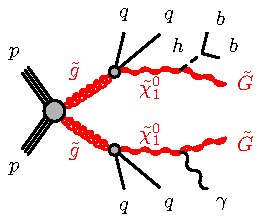
\includegraphics[width=0.5\textwidth]{images/analysis/gogo-qqqqbbphGG-h.pdf}
  \caption{Posible cadena de decaimiento del modelo supersimétrico en el que se centra esta Tesis.}
  \label{fig:phb_feyn}
\end{figure}

En la Sección \ref{sec:susy} se describe al MSSM juntos con la gran cantidad de parámetros que lo caracteriza. Cuando se desea generar muestras para un modelo, se debe elegir valores para esos parámetros que a priori son arbitrarios, y cuya única posible elección son los distintos objetivos del análisis. A su vez, se busca que al seleccionar valores para esos parámetros, tener el compromiso de no ser muy específicos con esos valores, ya que de esa forma el análisis terminaría siendo demasiado dedicado a un modelo particular. Ni tampoco muy arbitrarios, ya que se busca seguir manteniendo de alguna forma la fenomenología del mismo. Lo que se hace entonces es reducir los parámetros que caracterizan al modelo a unos pocos, y utilizar distintos programas de calculo que se encargan a partir de ellos generar tanto el espectro completo de masas, como los distintos posibles decaimientos de cada partícula.

El parámetro característico de este modelo es el $\mu$, el cual se elige negativo para habilitar el decaimiento del \ninoone a higgs. A su vez se desea anular el decaimiento al bosón $Z$, y que el decaimiento a fotones sea igual al de higgs, y para ello se eligió el valor óptimo de $M_1\sim -\mu$ \tosolve{Acá había encontrado una fórmula mediante un fit para M(mu), pero no se si es importante}. Con estos valores fue posible reducir el decaimiento al bosón $Z$ hasta casi un 10\%, dejando a los otros dos decaimientos aproximadamente en un 45\% como muestra la Figura \ref{fig:n1_br}. Como el modelo es un GGM, se fijó la masa del \gravino en $1$ eV \tosolve{esto no es tan así, la masa variaba de acuerdo al mu, lo deberia poner?}. 

\begin{figure}
  \centering
  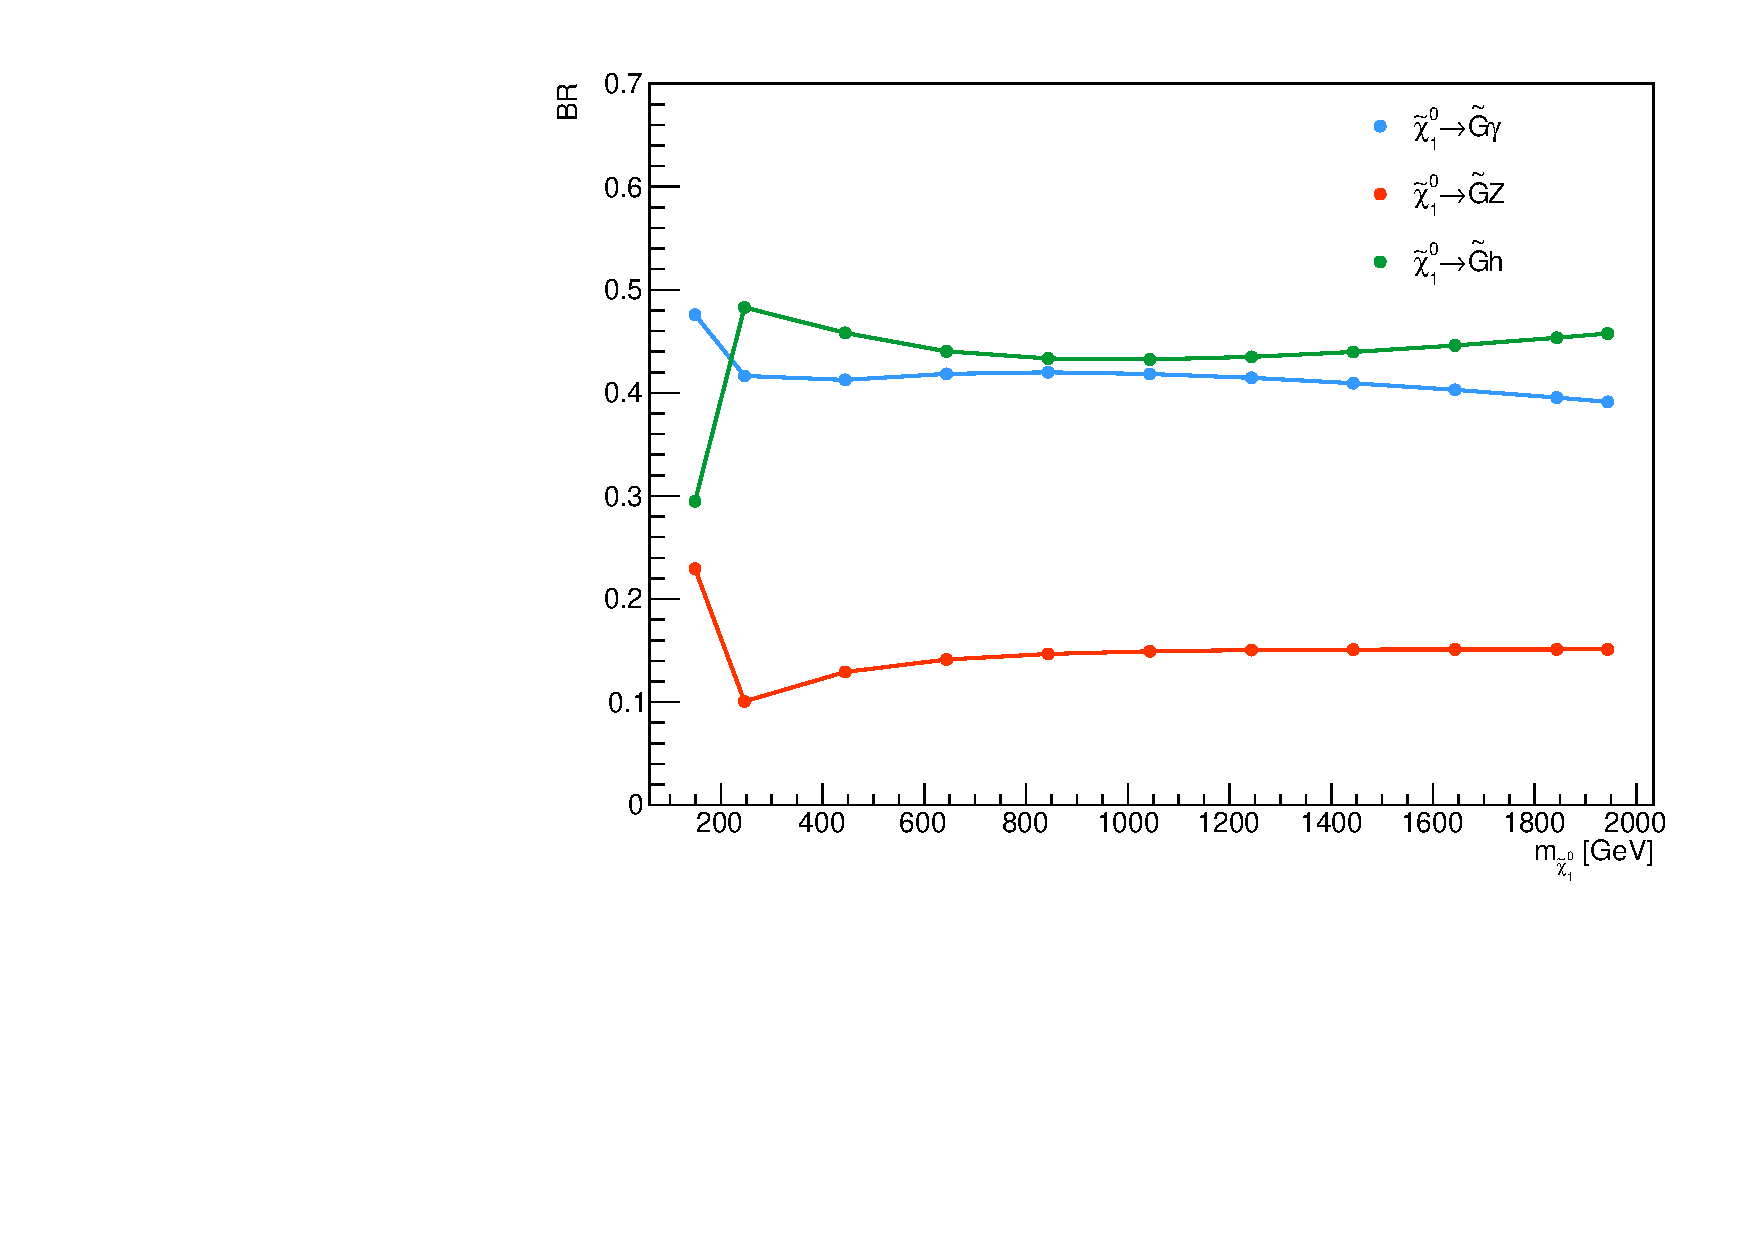
\includegraphics[width=0.6\textwidth]{images/analysis/phb_n1_br.pdf}
  \caption{Fracción de decaimiento del \ninoone en función de la masa del mismo.}
  \label{fig:n1_br}
\end{figure}

Las muestras fueron generadas considerando solamente la producción de gluinos a partir de la colisión $pp$. Además se eligió al gluino como la única partícula supersimétrica de color relevante, por lo que las masas de los squarks fueron fijadas a $5$ TeV, evitando así toda posible producción de los mismos. Los gluinos producidos en la colisión podían decaer un par de quark-antiquark más algún gaugino como se muestra en la Ecuación \ref{eq:gluino_dec}. Esto ocurre mediante squarks virtuales los cuales son completamente degenerados, pudiendo ser cualquiera de los 12 estados de sabor/quiralidad.

Además, se fijo a $M_2=3\ \tev$ y a $\tan{\beta}=1.5$ \tosolve{motivos formales?}. Todos los términos de acoplamiento trilineal fueron fijados a 0. Se eligió a la masa de los sleptons igual a $5$ TeV, para evitar así su producción la cual es estudiada por otros análisis. El bosón de higgs tiene una masa igual a la medida por las colaboraciones ATLAS y CMS \cite{higgs_mass}, $m_h=125\ \gev$, y sus decaimientos son elegidos de acuerdo a las predicciones del SM \tosolve{es asi?}, donde el predominante con un $\sim58$\% es a dos $b$-jets.
Adicionalmente se pone al mismo en el régimen de desacoplamiento con $m_A = 2\ \tev$. Al \ninoone se le fija su vida media, $c\tau_{\text{NLSP}}<0.1$ mm, de tal forma de que decaiga rápidamente  para que su vértice no esté muy desplazado del punto de colisión. Finalmente se anularon los decaimientos directos de los gluinos, charginos y neutralinos 1, 2 y 3. 

\tosolve{mencionar decaimientos masas de los demas neutralnos y charginos}

Debido a que son varios los análisis que estudian la producción de gluinos, la colaboración ATLAS puso a disposición unos archivos comunes a todos los análisis donde ya tiene almacenada la información de varios eventos de producción de gluinos. Estos archivos se denominan Les Houches Event (LHE), que le ahorran a cada análisis esta etapa de simulación, y sólo le resta generar las cadenas de decaimiento de los gluinos de acuerdo a sus modelos. En el presente análisis se omitieron correcciones radiativas así la masa de los los gluinos coincidía con el parámetro $M_3$, pudiendo así coincidir con los archivos LHE que están en función de la masa del mismo.

Los únicos parámetros libres del modelo son entonces $\mu$ y $M_3$ que determinan básicamente la masa de los \ninoone y gluinos. Se simularon 80 modelos distintos (puntos) con 10000 eventos en función de ambos parámetros, donde $150\ \gev<m_{\ninoone}<(m_{\tilde{g}}50)\ \gev$ y $1200\ \gev < m_{\tilde{g}}<2800\ \gev$. El arreglo completo de puntos de señal (grid) se puede observar en la Figura \ref{fig:grid_points}. Las muestras se realizaron con la simulación rápida del detector \textsc{ATLFAST-II} \tosolve{se supone que la voy a comentar en el segundo capitulo}. El espectro de masas completo, las fracciones de decaimiento de las sparticles y los anchos de decaimientos fueron calculados a partir del conjunto de parámetros anteriormente mencionados utilizando SUSPECT v2.43 \cite{Djouadi2007426}, SDECAY v1.5 \cite{Muhlleitner:2004mka} y HDECAY v3.4 \cite{Djouadi:1997yw}, que son parte del paquete SUSYHIT v1.5a \cite{Djouadi:2006bz}.
Como ejemplo se muestra en la Figura \ref{fig:mass_spec} un espectro de masas para unos de los puntos de señal con ($M_3$, $\mu$) = (1800 GeV, -1050 GeV). Un ejemplo de posibles decaimientos de los gluinos para ese mismo punto de señal se puede observar en la Figura \ref{fig:gluino_decays}. 

\begin{figure}
  \centering
  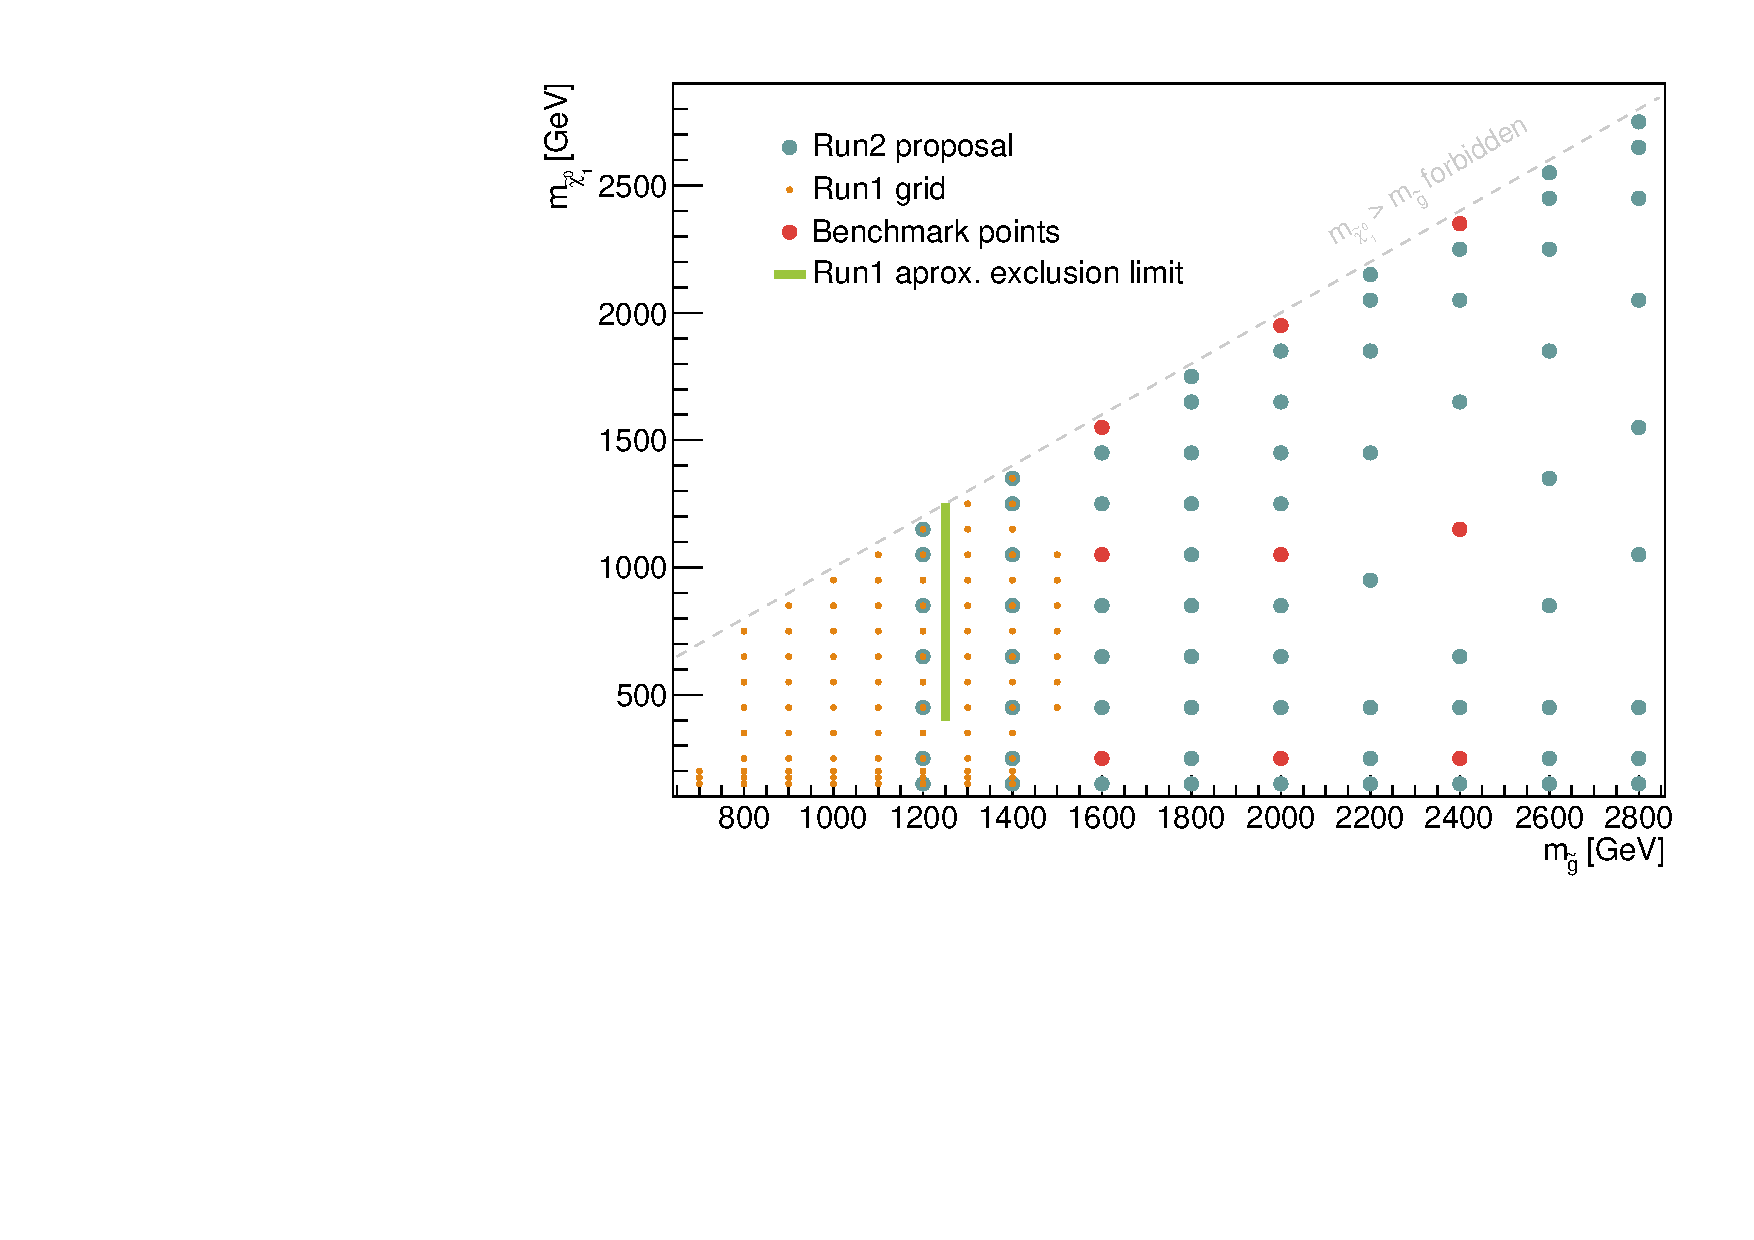
\includegraphics[width=0.6\textwidth]{images/analysis/phb_grid.pdf}
  \caption{Arreglo de muestras de señal generados en función de la masa del \ninoone y $\tilde{g}$. La densidad del mismo disminuye al aumentar $m_{\tilde{g}}$ debido a que la sensibilidad del análisis se estimó ser menor a los 2 TeV.}
  \label{fig:grid_points}
\end{figure}

\begin{figure}
  \centering
  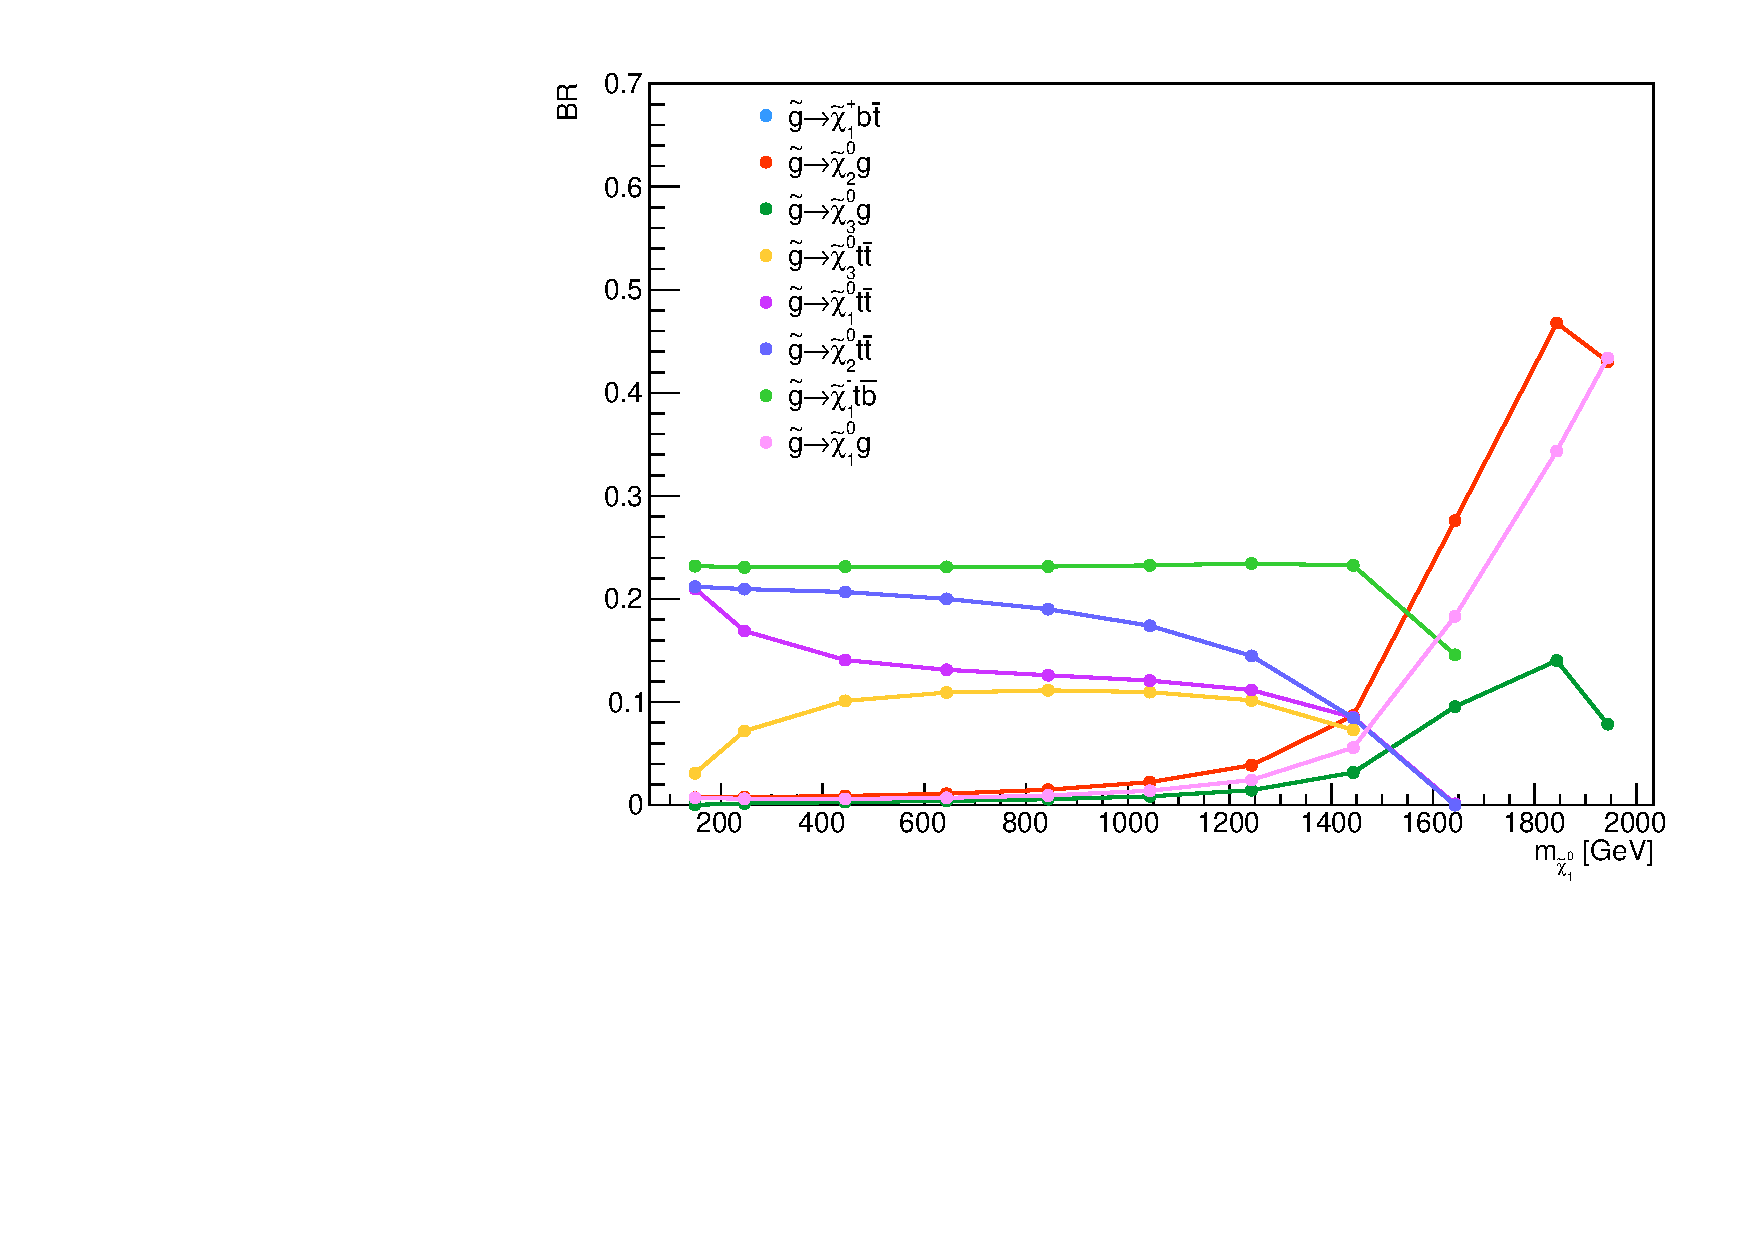
\includegraphics[width=0.6\textwidth]{images/analysis/phb_go_br.pdf}
  \caption{Fracción de decaimiento del gluino para el punto de señal con ($M_3$, $\mu$) = (1800 GeV, -1050 GeV). \tosolve{no sé si es necesario este plot...}}
  \label{fig:gluino_decays}
\end{figure}

\begin{figure}
  \centering
  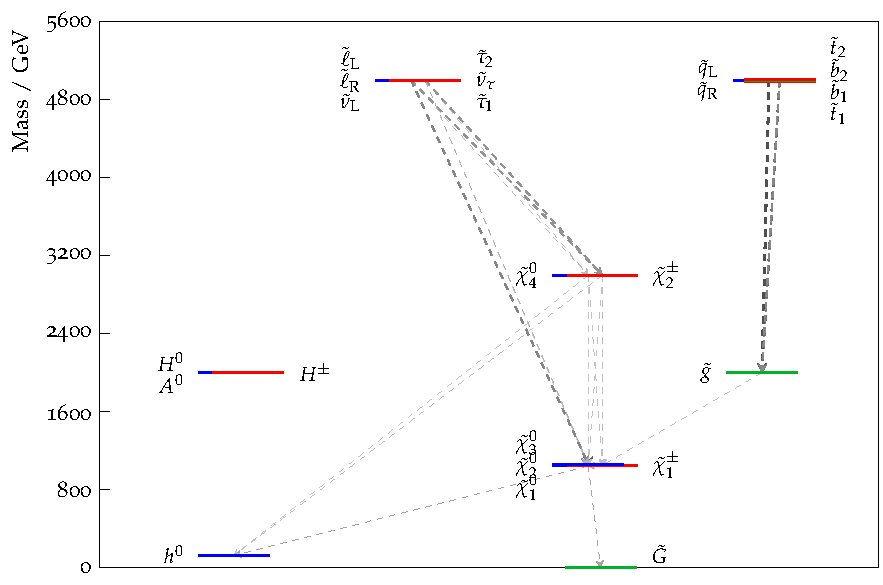
\includegraphics[width=0.6\textwidth]{images/analysis/phb_mass_spectrum.pdf}
  \caption{Espectro de masas de las sparticles para el punto de señal con ($M_3$, $\mu$) = (1800 GeV, -1050 GeV). \tosolve{hay una versión mejor de esta imagen}}
  \label{fig:mass_spec}
\end{figure}


\tosolve{Hay mas graficos de BR para poner, hacen falta? no lo creo...}

\section{Fondos del Modelo Estándar}


Los procesos del SM que son de interés como fondo para el análisis son aquellos que tienen un estado final igual al de la señal: fotones, jets y energía transversa faltante. Los mismos pueden clasificarse en distintos tipos. Por un lado, los procesos que dan lugar a eventos con un fotón y energía faltante real, es decir, los que se llaman fondos irreducibles. En este caso la energía la faltante proviene de los neutrinos, por lo que se componen principalmente de partículas que decaen a ellos, junto con fotones y jets de la ISR. Los procesos que cumplen con estos requisitos son la producción de bosones $Z$, $W$ y pares de top quarks que decaen subsecuentemente a bosones $W$:

\begin{itemize}
  \item $Z(\rightarrow \nu\nu) + \gamma + \text{jets}$
  \item $Z(\rightarrow \nu\nu) + \gamma + \gamma + \text{jets}$
  \item $W(\rightarrow l\nu) + \gamma + \text{jets}$
  \item $W(\rightarrow l\nu) + \gamma + \gamma + \text{jets}$
  \item $t\bar{t} + \gamma + \text{jets}$
\end{itemize}

Por otro lado es posible tener procesos que si bien no se producen fotones, unos de los objetos presentes en el mismo sea erróneamente reconstruido como tal, y genere un estado final igual al buscado pero con fotones `falsos'. Los objetos que pueden ser erróneamente reconstruidos como fotones en este caso pueden ser electrones o jets, por lo que hay que considerar aquellos procesos en los que se produzcan junto a neutrinos. Estos pueden ser:

\begin{itemize}
  \item $Z(\rightarrow \nu\nu) + \text{jets}$
  \item $W(\rightarrow l\nu) + \text{jets}$
  \item $t\bar{t} + \text{jets}$
\end{itemize}

Por último, puede ocurrir que si bien en el proceso no hayan neutrinos, una reconstrucción errónea de la energía de los distintos objetos presentes en el evento genere un desbalance a la hora de calcular la energía transversa faltante, y por ende tengan una cantidad no despreciable de la misma denominada energía transversa faltante instrumental. Este tipo de eventos puede ocurrir también en simultáneo junto con fotones `falsos', por lo que existen diversos procesos que cumplan estos requisitos, entre ellos se encuentran:

\begin{itemize}
  \item jets (denominado Multijet o QCD)
  \item $\gamma + \text{jets}$
  \item $\gamma + \gamma + \text{jets}$
  \item $Z(\rightarrow ll) + \text{jets}$
  \item $Z(\rightarrow ll) + \gamma + \text{jets}$
  \item $Z(\rightarrow ll) + \gamma + \gamma + \text{jets}$
\end{itemize}

A partir de aquí, como notación simplificada de los fondos del análisis, se omite en el nombre tanto el `+' como la producción de jets en la ISR. Cabe destacar que existen más procesos que cumplen las condiciones anteriores pero que no fueron considerados para el análisis. Lo que ocurre con ellos es que la sección eficaz es demasiado baja o el estado final tiene una cinemática muy fácil de suprimir por las selecciones básicas del análisis, por lo que su contribución es completamente despreciable. Algunos ejemplos de ellos son la producción doble de bosones  ($WW$, $ZZ$, $WZ$), bosones decayendo a quarks ($W(\rightarrow qq)$, $Z(\rightarrow qq)$), producción de top ($t\gamma$, $tW$), entre otros.

Para modelar los fondos con fotones `reales' se utilizaron simulaciones de MC, mientras que para aquellos con fotones `falsos' se utilizaron técnicas basadas en datos. \tosolve{mencionar que para la optimizacion sí se usaron MC para los fakes?}. Para los jets falseando fotones se utilizó un método denominado \texttt{ABCD}, y para los electrones falseando fotones un método denominado \texttt{Tag\&Probe}. El modelado de todos los fondos se describe en las siguientes Secciones.

\subsection{Muestras de fondo a partir de simulaciones de Monte Carlo}

Los fondos del SM con fotones `reales' fueron modelados utilizando simulaciones de MC, los cuales consisten en: \phj, \wph, \ttbarph, \wphph, \zph, \zphph, \phph. Los tres primeros son considerados los de mayor impacto en el análisis y por ende fueron normalizados en respectivas regiones de control. Para el resto de los fondos se utilizaron las simulaciones con las normalizaciones usuales. 
Cabe mencionar que también el fondo \znunuph es considerado de alta importancia en el análisis, pero la dificultad para diseñar una región de control dedicada llevó a la decisión de utilizarlo con las normalizaciones usuales. La parte del análisis que se basa en la producción electrodébil  sí hace uso de una región de control dedicada para este análisis, y se describe en el Capítulo \ref{cap:analysis_EWK}.

Todos los procesos salvo \ttbarph fueron simulador utilizando el generador \texttt{SHERPA} v2.2 \cite{Bothmann:2019yzt}. Los elementos de la matriz se calculan para un máximo de cuatro partones
a LO y se fusionan con la lluvia de partones de \texttt{SHERPA} \cite{Schumann:2007mg} utilizando la prescripción de \texttt{MEPS@LO} \cite{Hoeche:2012yf}. La muestra de \ttbarph se genera con \texttt{MadGgraph5\_aMC@NLO} \cite{Alwall:2014hca} a segundo orden en teoría de perturbaciones (NLO), con \texttt{Pythia8} para el modelo de la lluvia de partones \cite{Sjostrand:2014zea}. \tosolve{algún dato más debería poner, cual?}. En la Tabla \ref{tab:mc_samples} se muestran todas las muestras de fondos utilizadas en el análisis, las mismas se encuentras segmentadas (\textit{slicing}) de acuerdo a diferentes criterios.

\begin{table}[h!]
  \centering
  \caption{Muestras de fondos de MC utilizadas en el análisis, donde se especifica su generador, sección eficaz, $k$-factor y eficiencia de filtro.}
  \label{tab:mc_samples}
  \resizebox{\textwidth}{!}{
  \begin{tabular}{llrrr}

     \hline
      \hline
    Proceso & Generador & Sección Eficaz [pb] & $k$-factor & Eficiencia de filtro \\

    \hline
     \hline

    \ttbarph, $\pt^{\gamma} > 140$ \gev  & \texttt{MadGgraph5\_aMC@NLO}/\texttt{Pythia8} & 0.21551  & 1.0 & 1.0  \\

    \hline

    $Z(ee)\gamma$, $\pt^\gamma>140$ \gev                 & \texttt{SHERPA} v2.2.2 & 0.0634   & 1.0 & 1.0\\
    $Z(\mu\mu)\gamma$, $\pt^\gamma>140$ \gev             & \texttt{SHERPA} v2.2.2 & 0.0632   & 1.0 & 1.0\\

    $Z(\tau\tau)\gamma$, $\pt^\gamma>140$ \gev           & \texttt{SHERPA} v2.2.2 & 0.0634   & 1.0 & 1.0\\

    $Z(\nu\nu)\gamma$, $\pt^\gamma>140$ \gev             & \texttt{SHERPA} v2.2.2 & 0.2446   & 1.0 & 1.0\\

  \hline
    $W(e \nu)\gamma$, $\pt^\gamma>140$ \gev              & \texttt{SHERPA} v2.2.2 & 0.2980   & 1.0 & 1.0\\


    $W(\mu \nu)\gamma$, $\pt^\gamma>140$ \gev            & \texttt{SHERPA} v2.2.2 & 0.2987   & 1.0 & 1.0\\


    $W(\tau \nu)\gamma$, $\pt^\gamma>140$ \gev           & \texttt{SHERPA} v2.2.2 & 0.2983   & 1.0 & 1.0\\
    \hline
    \phj, $\pt^\gamma \in [70-140]$ \gev      & \texttt{SHERPA} v2.2.2 & 4526.5   & 1.0 & 1.0 \\
    \phj, $\pt^\gamma \in [140-280]$ \gev     & \texttt{SHERPA} v2.2.2 & 376.05   & 1.0 & 1.0 \\
    \phj, $\pt^\gamma \in [280-500]$ \gev     & \texttt{SHERPA} v2.2.2 & 21.851   & 1.0 & 1.0 \\
    \phj, $\pt^\gamma \in [500-1000]$ \gev    & \texttt{SHERPA} v2.2.2 & 1.4637   & 1.0 & 1.0 \\
    \phj, $\pt^\gamma \in [1000 - ]$ \gev       & \texttt{SHERPA} v2.2.2 & 0.02987  & 1.0 & 1.0 \\
    \hline
    \phph, $m_{\gamma\gamma} \in [0-50]     $ \gev         & \texttt{SHERPA} v2.2.4 & 93.499                 & 1.0 & 1.0 \\
    \phph, $m_{\gamma\gamma} \in [50-90]    $ \gev         & \texttt{SHERPA} v2.2.4 & 139.04                 & 1.0 & 1.0 \\
    \phph, $m_{\gamma\gamma} \in [90-175]   $ \gev         & \texttt{SHERPA} v2.2.4 & 51.818                 & 1.0 & 1.0 \\
    \phph, $m_{\gamma\gamma} \in [175-2000] $ \gev         & \texttt{SHERPA} v2.2.4 & 10.999                 & 1.0 & 1.0 \\
    \phph, $m_{\gamma\gamma} \in [2000-]    $ \gev         & \texttt{SHERPA} v2.2.4 & 0.0007                 & 1.0 & 1.0 \\
      \hline
      $Z(ee)\gamma\gamma$,      $\pt^{\text{sub}-\gamma} \in [9-17]$ \gev                 &  \texttt{SHERPA} v2.2.4 & $0.8705$ & 1.0 & 1.0 \\
      $Z(ee)\gamma\gamma$,      $\pt^\gamma>17$ \gev, $m_{\gamma\gamma} \in [0-80]$ \gev  &  \texttt{SHERPA} v2.2.4 & $0.1993$ & 1.0 & 1.0 \\
      $Z(ee)\gamma\gamma$,      $\pt^\gamma>17$ \gev, $m_{\gamma\gamma}>80$ \gev          &  \texttt{SHERPA} v2.2.4 & $0.0345$ & 1.0 & 1.0 \\

      $Z(\mu\mu)\gamma\gamma$,  $\pt^{\text{sub}-\gamma} \in [9-17]$ \gev                 &  \texttt{SHERPA} v2.2.4 & $0.8689$ & 1.0 & 1.0 \\
      $Z(\mu\mu)\gamma\gamma$,  $\pt^\gamma>17$ \gev, $m_{\gamma\gamma} \in [0-80]$ \gev  &  \texttt{SHERPA} v2.2.4 & $0.1999$ & 1.0 & 1.0 \\
      $Z(\mu\mu)\gamma\gamma$,  $\pt^\gamma>17$ \gev, $m_{\gamma\gamma}>80$ \gev          &  \texttt{SHERPA} v2.2.4 & $0.0346$ & 1.0 & 1.0 \\

      $Z(\tau\tau)\gamma\gamma$,$\pt^{\text{sub}-\gamma} \in [9-17]$ \gev                 &  \texttt{SHERPA} v2.2.4 & $0.8718$ & 1.0 & 1.0 \\
      $Z(\tau\tau)\gamma\gamma$,$\pt^\gamma>17$ \gev, $m_{\gamma\gamma} \in [0-80]$ \gev  &  \texttt{SHERPA} v2.2.4 & $0.2005$ & 1.0 & 1.0 \\
      $Z(\tau\tau)\gamma\gamma$,$\pt^\gamma>17$ \gev, $m_{\gamma\gamma}>80$ \gev          &  \texttt{SHERPA} v2.2.4 & $0.0345$ & 1.0 & 1.0 \\

      $Z(\nu\nu)\gamma\gamma$,  $\pt^{\text{sub}-\gamma} \in [9-17]$ \gev                 &  \texttt{SHERPA} v2.2.4 & $0.0919$ & 1.0 & 1.0 \\
      $Z(\nu\nu)\gamma\gamma$,  $\pt^\gamma>17$ \gev, $m_{\gamma\gamma} \in [0-80]$ \gev  &  \texttt{SHERPA} v2.2.4 & $0.0237$ & 1.0 & 1.0 \\
      $Z(\nu\nu)\gamma\gamma$,  $\pt^\gamma>17$ \gev, $m_{\gamma\gamma}>80$ \gev          &  \texttt{SHERPA} v2.2.4 & $0.0184$ & 1.0 & 1.0 \\
      \hline
      $W(e\nu)\gamma\gamma$,    $\pt^{\text{sub}-\gamma} \in [9-17]$ \gev                 &  \texttt{SHERPA} v2.2.4 & $0.4396$ & 1.0 & 1.0 \\
      $W(e\nu)\gamma\gamma$,    $\pt^\gamma>17$ \gev, $m_{\gamma\gamma} \in [0-80]$ \gev  &  \texttt{SHERPA} v2.2.4 & $0.0715$ & 1.0 & 1.0 \\
      $W(e\nu)\gamma\gamma$,    $\pt^\gamma>17$ \gev, $m_{\gamma\gamma}>80$ \gev          &  \texttt{SHERPA} v2.2.4 & $0.0379$ & 1.0 & 1.0 \\

      $W(\mu\nu)\gamma\gamma$,  $\pt^{\text{sub}-\gamma} \in [9-17]$ \gev                 &  \texttt{SHERPA} v2.2.4 & $0.4384$ & 1.0 & 1.0 \\
      $W(\mu\nu)\gamma\gamma$,  $\pt^\gamma>17$ \gev, $m_{\gamma\gamma} \in [0-80]$ \gev  &  \texttt{SHERPA} v2.2.4 & $0.0711$ & 1.0 & 1.0 \\
      $W(\mu\nu)\gamma\gamma$,  $\pt^\gamma>17$ \gev, $m_{\gamma\gamma}>80$ \gev          &  \texttt{SHERPA} v2.2.4 & $0.0379$ & 1.0 & 1.0 \\

      $W(\tau\nu)\gamma\gamma$, $\pt^{\text{sub}-\gamma} \in [9-17]$ \gev                 &  \texttt{SHERPA} v2.2.4 & $0.4373$ & 1.0 & 1.0 \\
      $W(\tau\nu)\gamma\gamma$, $\pt^\gamma>17$ \gev, $m_{\gamma\gamma} \in [0-80]$ \gev  &  \texttt{SHERPA} v2.2.4 & $0.0715$ & 1.0 & 1.0 \\
      $W(\tau\nu)\gamma\gamma$, $\pt^\gamma>17$ \gev, $m_{\gamma\gamma}>80$ \gev          &  \texttt{SHERPA} v2.2.4 & $0.0379$ & 1.0 & 1.0 \\
    \hline
     \hline
  \end{tabular}
  }
\end{table}

\subsection{Fondo de jets erróneamente reconstruidos como fotones}

Es posible que un jet sea erróneamente reconstruido como un fotón principalmente cuando proviene de un $\pi^0$. Los piones neutrales decaen rápidamente a dos fotones que naturalmente son reconstruidos en el ECAL. Para poder distinguir el decaimiento de un pión de la producción de un fotón individual utiliza la primera capa del calorímetro, que tiene mayor granularidad (Sección \ref{sec:ph_id}). En el caso de que el pión se produzca con un elevado \pt, los dos fotones pueden estar muy colimados y por ende ser prácticamente indistinguibles de un fotón individual. Si bien la identificación \texttt{Tight} se encarga se suprimir en gran parte esta reconstrucción errónea, aún así puede contener una contaminación moderada de este proceso. Este tipo de fondo proviene principalmente de procesos como Multijets, $W+\text{jets}$ o de \ttbar decayendo semi-leptónicamente. Esta reconstrucción errónea de jets no es esperable que sea modelada correctamente mediante simulaciones de MC, por lo que se utilizan técnicas basadas en datos para modelarla.

El método empleado para estimar este fondo se denomina \texttt{ABCD} \cite{Alonso:2233238}. El mismo hace uso de la diferencia que existe en las distribuciones de aislamiento de fotones `reales' (señal en este contexto) y la de los `falsos' (fondo), para poder selecciones eventos de uno u otro \tosolve{Esto cuando se utilizaría? Me parece que mirar las formas quedó de un método viejo no? Ahora solo miramos número de eventos. O es para la correlación?}. En el contexto de este método se definen fotones aislados como aquellos que pasan el WP \texttt{FixedCutTight} \tosolve{esta bien esto?}, $-20\ \gev<\ETiso<0\ \gev$ y $0<\pTiso<0.05$, y los no-aislados aquellos con $8\ \gev<\ETiso<80\ \gev$ o $0.15<\pTiso<1$ \tosolve{capaz deba definir estas variables aca, o en la parte de fotones}. A su vez se utiliza una selección de identificación adicional que discrimina los fotones `reales' \texttt{Tight} de los fotones `falsos'. Este criterio de identificación se denomina \texttt{Non-Tight} (también \textit{pseudo-photons}, \texttt{Tight-4} o \texttt{LoosePrime}) y consiste en los fotones que pasan la selección \texttt{Loose} y que además fallan alguno de los criterios de selección \texttt{Tight} que emplea las variables $w_{s3}$, $F_{\text{side}}$, $\Delta E$, $E_{\text{ratio}}$. Por lo que esta selección es un subconjunto de los eventos seleccionados por el trigger de fotones loose pero ortogonal a la identificación \texttt{Tight}. 

El método \texttt{ABCD} preselecciona eventos con al menos un fotón con $\pt>1450\ \gev$, al menos dos jets y ningún leptón, cuyos requisitos son idénticos a los que se usan en el análisis descriptos en la Sección \ref{sec:selection}. A partir de ello define cuatro regiones \cite{ATL-COM-PHYS-2016-1626}:

\begin{itemize}
  \item Región A: fotones \texttt{Tight} y aislados
  \item Región B: fotones \texttt{Tight} y no aislados
  \item Región C: fotones \texttt{Non-Tight} y aislados
  \item Región D: fotones \texttt{Non-Tight} y no aislados
\end{itemize}

La Figura \ref{fig:abcd_regions} muestra la distribución de datos en las variables de aislamiento para las regiones A, B, C y D. En la misma se ve explícita la brecha (\textit{gap}) que existe entre las variables de aislamiento para reducir así la contaminación entre las regiones \tosolve{es por esto?}.

\begin{figure}
  \centering
  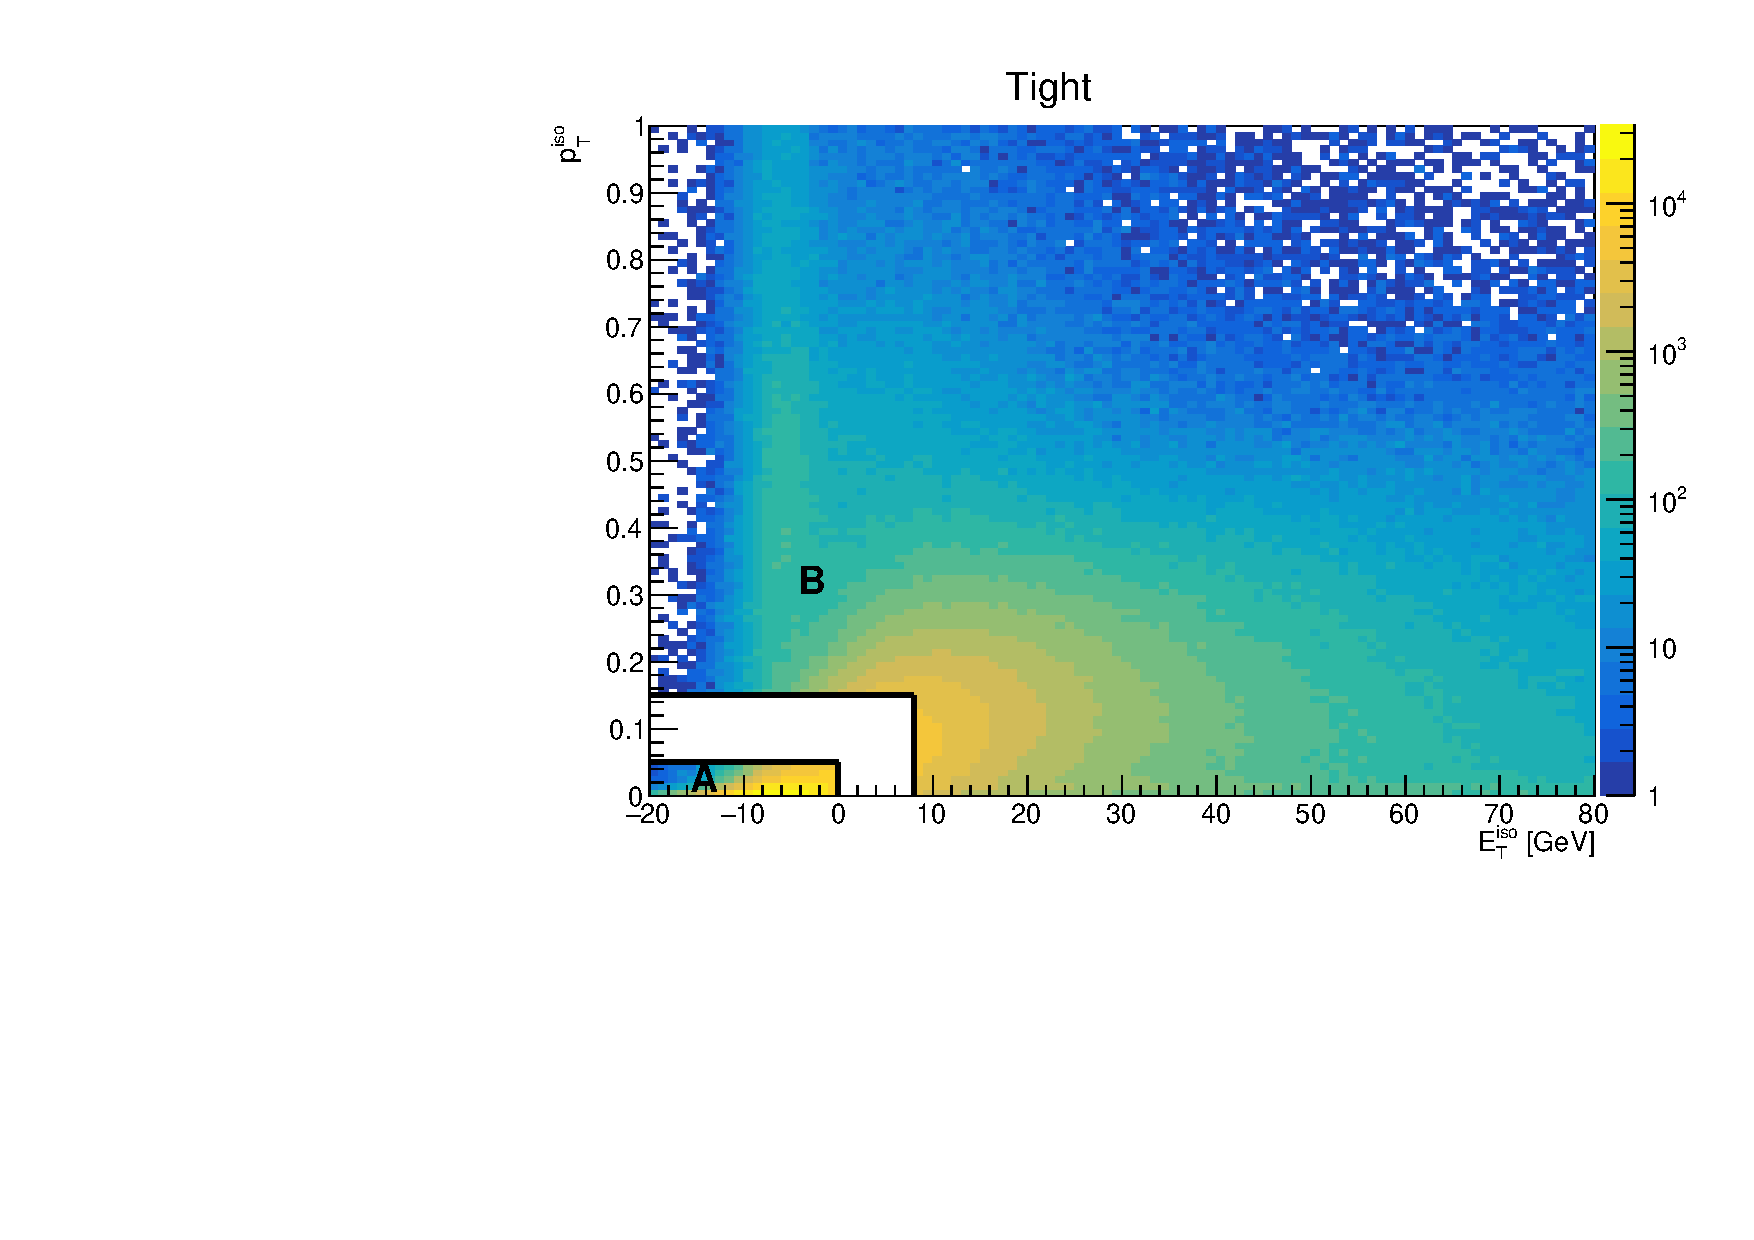
\includegraphics[width=0.45\textwidth]{images/analysis/tight_ABCD_data.pdf}
  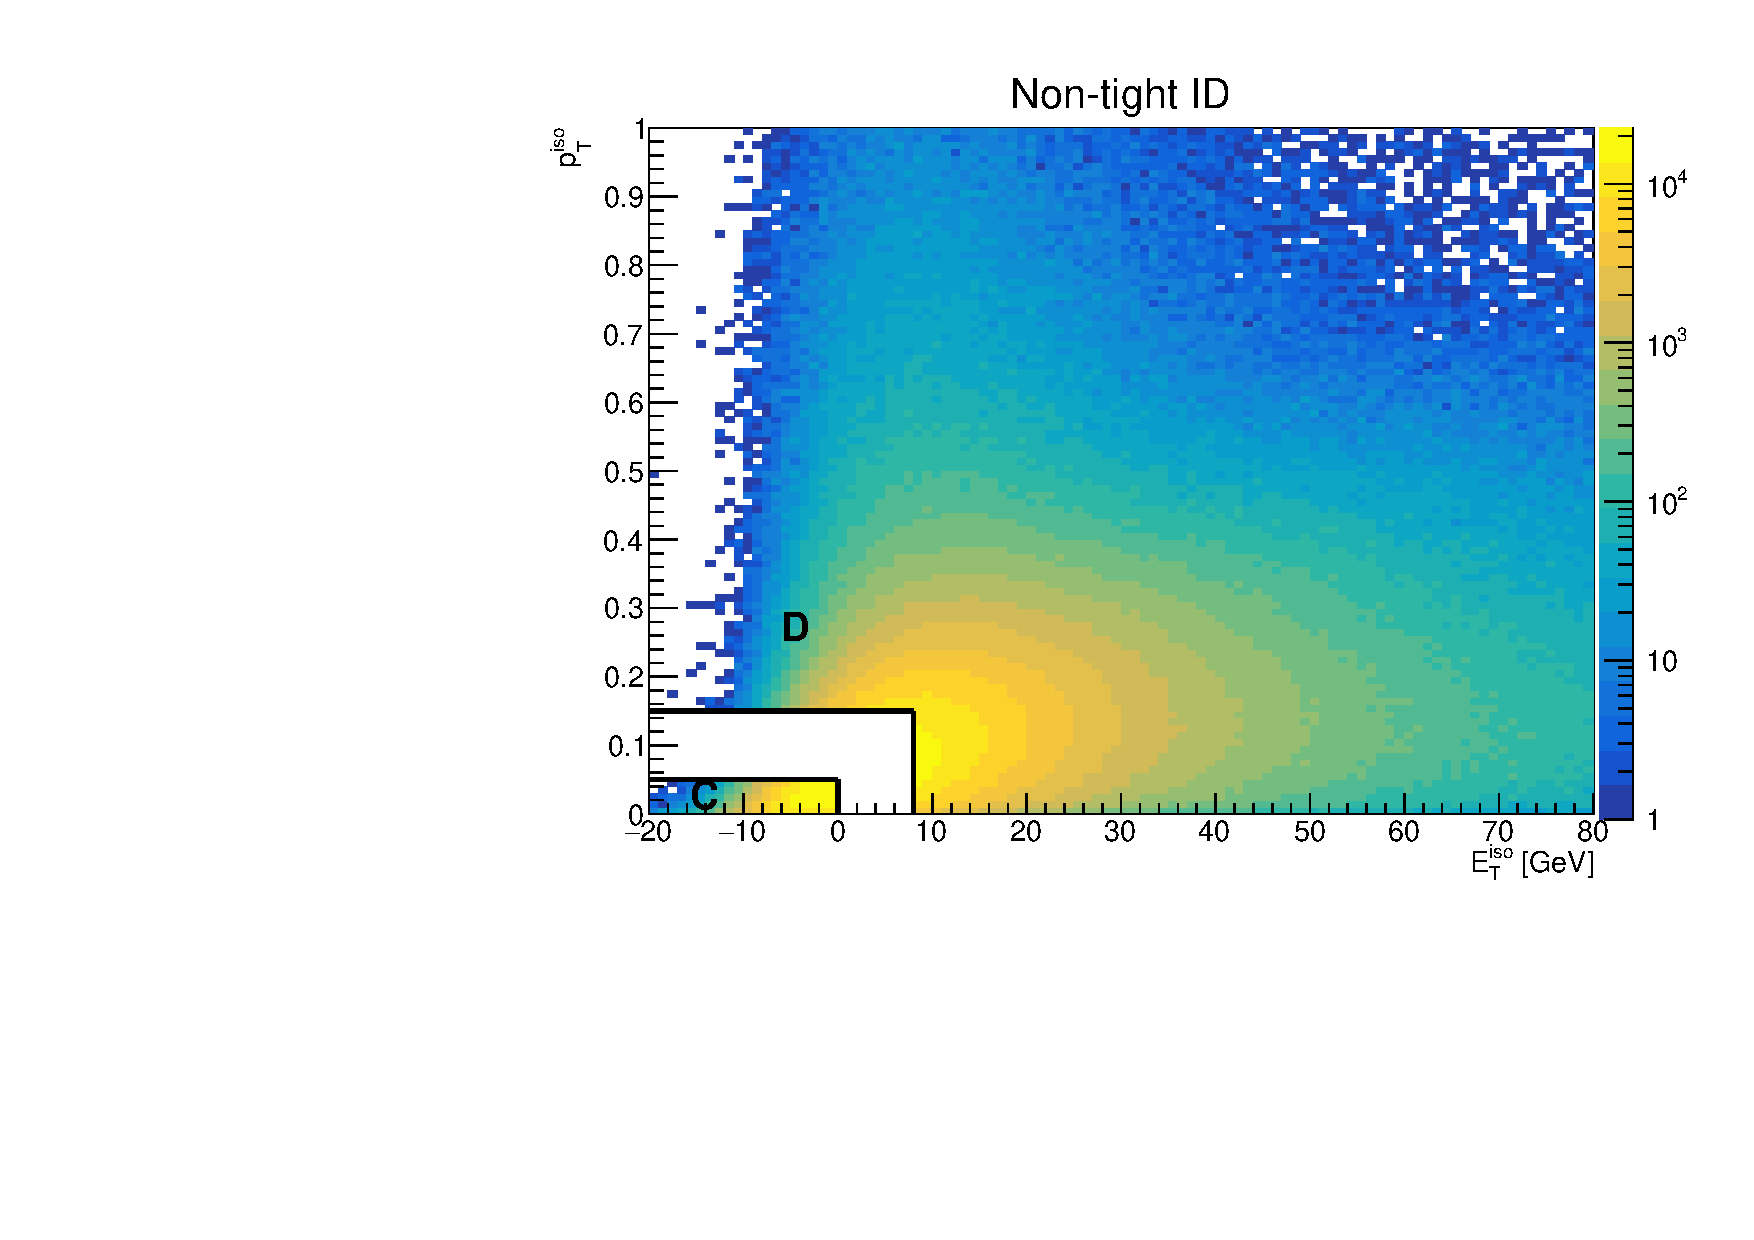
\includegraphics[width=0.45\textwidth]{images/analysis/nontight_ABCD_data.pdf}
  \caption{Distribución de datos en las variables de aislamiento para las regiones A, B, C y D.}
  \label{fig:abcd_regions}
\end{figure}


El método se basa en asumir que no hay correlación entre las variables de aislamiento y la selección de identificación \cite{tesis_tony}, y que tampoco hay contaminación de eventos de señal en las regiones B, C y D ($N_{B,C,D}^b=N_{B,C,D}$), lo que permite esperar la siguiente relación $N_A^b/N_B=N_C/N_D$. 
% Donde cada término representa el número de fondo en cada región. 
Reescribiendo la expresión anterior se puede estimar el número de fondo en la región A como:

\begin{equation}
  N_A^b = \text{FF}_{\text{iso}}\times N_B = \text{FF}_{\text{ID}}\times N_C
  \label{eq:jfakes_ff}
\end{equation}
%
donde:
\begin{equation}
  \begin{split}
    \text{FF}_{\text{iso}} &= \frac{N_C}{N_D} \\
    \text{FF}_{\text{ID}} &= \frac{N_B}{N_D} \\
  \end{split}
\end{equation}
%
denominados \textit{fake factors} (FF). 
Si bien ambos factores deberían dar resultado equivalente, se encontró que al usar $\text{FF}_{\text{iso}}$ las incertidumbres sistemáticas se veían reducidas, y por ende se decidió usar al mismo en el análisis.

Distintas correcciones se realizan sobre este método. El primero es considerar que efectivamente hay una contaminación de señal en las regiones B, C y D. La misma es estimada utilizando simulaciones de MC con fotones `reales' a nivel generador, y restada a los datos observados en cada región. Adicionalmente se consideró que podría llegar a haber una correlación entre variables calorimétricas y de identificación, que se puede agregar como un factor multiplicativo a la Ecuación \ref{eq:jfakes_ff}. Ese factor se define como:

\begin{equation}
  R = \frac{N_a^b N_D^b}{N_B^b N_C^b} \neq 1
\end{equation}

Debido al blinding del análisis, no es posible conocer el número de eventos en la región A, por lo que se calcula el factor $R$ en regiones distintas pero asumiendo que tienen la misma correlación entre ellas:

\begin{equation}
  R' = \frac{N_a' N_D'}{N_B' N_C'} \neq 1
\end{equation}
%
donde:
\begin{itemize}
  \item Región A: fotones \texttt{Tight}, $9\ \gev<\ETiso<15\ \gev$ y $0.2<\pTiso<0.3$
  \item Región B: fotones \texttt{Tight}, $15\ \gev<\ETiso<80\ \gev$ y $0.3<\pTiso<1$
  \item Región C: fotones \texttt{Non-Tight}, $9\ \gev<\ETiso<15\ \gev$ y $0.2<\pTiso<0.3$
  \item Región D: fotones \texttt{Non-Tight}, $15\ \gev<\ETiso<80\ \gev$ y $0.3<\pTiso<1$
\end{itemize}
%
cuyas definiciones apuntan a tener regiones con fondo exclusivamente pero con estadística suficiente.

Con estas correcciones la estimación del fondo queda de la forma:

\begin{equation}
    N_{\jfake} = N_A^b = \left[R' \frac{N_C - N_C^s}{N_D - N_D^s} \left( 1 - \frac{N_B^s}{N_B} \right)  \right] \times N_B = \text{FF}_{\text{iso}} \times N_B \\
\end{equation}

Los FFs fueron estimados en función del \pt y $|\eta|$ del fotón, y la \met del evento. Distintas fuentes de incertidumbre sistemática fueron consideradas. Una fue cambiar la definición de la identificación \texttt{Non-Tight} utilizando ahora \texttt{Tight-3} (fallando ahora $w_{s3}$, $F_{\text{side}}$ o $\Delta E$) y \texttt{Tight-5} ($w_{s3}$, $F_{\text{side}}$, $\Delta E$, $E_{\text{ratio}}$ o $w_{\text{stot}}$). A su vez se consideró los efectos de la correlación residual calculado los FFs con $R'=1$ e incluyéndolos como sistemático.

En la Tabla \ref{tab:jfake_ff} se puede observar los valores de los FFs obtenidos en función del \pt y $|\eta|$ del fotón, y la \met del evento. Los valores obtenidos para $R'$ dieron cercanos a la unidad con desviaciones cercanas al 10\%.

\begin{table}[!ht]
  \centering
  \caption{Valores obtenidos para los factores de reconstrucción errónea de jets en fotones en función del \pt y $|\eta|$ del fotón, y la \met del evento. Las incertidumbres son tanto estadísticas como sistemáticas.}
  \resizebox{.6\textwidth}{!}{
  \begin{tabular}{c|l|ccc}
    \hline
    \hline
      \multirow{2}{*}{$|\eta|$} & \multirow{2}{*}{{\pt} [{\gev}]}  & \multicolumn{3}{c}{\met [GeV]} \\
        & & $[50-100]$         & $[100-200]$        & $>200$              \\
    \hline
    \hline
    \multirow{6}{*}{Barrel}       & $[145-200]$   & 0.055 $\pm$ 0.0077 & 0.042 $\pm$ 0.0047 &  0.066 $\pm$ 0.0241 \\
  & $[200-250]$                      & 0.044 $\pm$ 0.0051 & 0.027 $\pm$ 0.0033 &  0.059 $\pm$ 0.0163 \\
  & $[250-300]$                      & 0.041 $\pm$ 0.0034 & 0.022 $\pm$ 0.0047 &  0.057 $\pm$ 0.0095 \\
  & $[300-350]$                      & 0.037 $\pm$ 0.0043 & 0.019 $\pm$ 0.0026 &  0.046 $\pm$ 0.014  \\
  & $[350-400]$                      & 0.036 $\pm$ 0.0033 & 0.019 $\pm$ 0.0035 &  0.057 $\pm$ 0.0117 \\
  & $>400$                           & 0.038 $\pm$ 0.0053 & 0.013 $\pm$ 0.0022 &  0.047 $\pm$ 0.011  \\

    \hline
    \multirow{6}{*}{End-cap}      & $[145-200]$                      & 0.048 $\pm$ 0.0152 & 0.053 $\pm$ 0.0139 & 0.213 $\pm$ 0.0963 \\
       & $[200-250]$                      & 0.045 $\pm$ 0.0114 & 0.041 $\pm$ 0.0102 & 0.226 $\pm$ 0.125  \\
   & $[250-300]$                      & 0.05  $\pm$ 0.0079 & 0.039 $\pm$ 0.0097 & 0.143 $\pm$ 0.043  \\
   & $[300-350]$                      & 0.052 $\pm$ 0.0085 & 0.03  $\pm$ 0.0058 & 0.08  $\pm$ 0.0515 \\
   & $[350-400]$                      & 0.058 $\pm$ 0.0071 & 0.043 $\pm$ 0.0079 & 0.179 $\pm$ 0.1064 \\
   & $>400$                           & 0.07  $\pm$ 0.0095 & 0.047 $\pm$ 0.0077 & 0.141 $\pm$ 0.0528 \\
    \hline
    \hline
  \end{tabular}
  }
  \label{tab:jfake_ff}
\end{table}




\subsection{Fondo de electrones erróneamente reconstruidos como fotones}

Los fotones y los electrones pueden dejan lluvias electromagnéticas muy
similares en el ECAL, y su reconstrucción se describió en la Sección \ref{sec:ph_el}.
Si bien los algoritmos de reconstrucción de electrones y fotones están diseñados para poder discriminar uno de otros, una pequeña fracción residual de electrones puede ser reconstruida erróneamente como fotón. Si bien la reconstrucción de los clusters es altamente efectiva, la fracción de electrones mal reconstruidos se debe prácticamente a ineficiencias en la reconstrucción de trazas. Por ejemplo, la traza de un electrón puede ser mal reconstruida como un vértice de conversión y por ende el mismo es reconstruido como un fotón convertido. O inclusive una errónea asociación de la traza con el cluster puede hacer que el electrón sea reconstruido como fotón no convertido.
Puede ocurrir a su vez que el cluster no pase los criterios de ambigüedad y el objeto sea almacenado por duplicado como electrón y fotón. Esto en general es fácil de suprimir aplicando requisitos de solapamiento, pero estos pueden favorecer al electrón y por ende tener en la selección del análisis nuevos electrones mal reconstruidos. Este tipo de efectos se ve principalmente en procesos como $W(l\nu)+\text{jets}$, $Z(ee)+\text{jets}$ o \ttbar. Nuevamente como es prácticamente imposible estimar esta reconstrucción errónea con simulaciones de MC, se utiliza una técnica basada en datos para estimar una fracción de reconstrucción errónea.

Para ello lo que se hace es utilizar una muestra e eventos con producción de bosón $Z$. Como el mismo no puede decaer a $e+\gamma$, los eventos con este par de partículas y que parecieran provenir del decaimiento de un $Z$ son un buen indicio de que ese fotón en realidad es un electrón mal reconstruido. En ese caso se puede estimar una fracción de reconstrucción errónea (fake factor, FF) como:

\begin{equation}
  F_{e\to \gamma} \equiv \frac{P(e^{\text{real}}\to \gamma^{\text{reco}})}{P(e^{\text{real}}\to e^{\text{reco}})}  = \frac{\epsilon(e^{\text{real}}\to \gamma^{\text{reco}})}{\epsilon(e^{\text{real}}\to e^{\text{reco}})} \frac{\epsilon^{\text{ID}}_{\gamma}}{\epsilon^{\text{ID}}_{e}} = \frac{N_{e^{\text{real}}\to \gamma^{\text{reco}}}}{N_{e^{\text{real}}\to e^{\text{reco}}}} \frac{\epsilon^{\text{ID}}_{\gamma}}{\epsilon^{\text{ID}}_{e}}
  \label{eq:efake_ff}
\end{equation} 
%
donde $P(e\to e(\gamma))$ es la probabilidad de reconstruir e identificar un electrón `real' como un electrón (fotón), $\epsilon(e^{\text{real}}\to e(\gamma)^{\text{reco}})$ es la eficiencia de reconstruir un electrón `real' como un electrón (fotón)\footnote{Definida como $\frac{N_{e^{\text{real}}\to e(\gamma)^{\text{reco}}}}{N_{e^{\text{real}}\to e^{\text{reco}}}+N_{e^{\text{real}}\to \gamma^{\text{reco}}}}$}, $\epsilon^{\text{ID}}_{e} (\epsilon^{\text{ID}}_{\gamma})$ es la eficiencia de identificar un electrón (fotón) y $N_{\text{real } e\to \text{reco } e(\gamma)}$ el número electrones reconstruidos como electrones (fotones). Como no es posible saber a partir de los datos cuándo un electrón es `real', este factor debe ser estimado a partir de los objetos ya reconstruidos y sus eficiencias, magnitudes que sí son mensurables en datos. Para una dada muestra con eventos de bosones $Z$, la probabilidad de reconstruir a sus productos de decaimiento como pares $ee$ o $e\gamma$ esta dada por \tosolve{tengo que pensar mejor estas fórmulas, pero va por aca la cosa}:

\begin{equation}
\frac{N_{ee}}{N_Z} = (\epsilon^{ID}_{e})^{2} (1-\epsilon(e^{\text{true}}\to \gamma^{\text{reco}}))^{2}
\quad
\frac{N_{e\gamma}}{N_Z} = \epsilon^{ID}_{e}\epsilon^{ID}_{\gamma} (1-\epsilon(e^{\text{true}}\to \gamma^{\text{reco}}))\epsilon(e^{\text{true}}\to \gamma^{\text{reco}})
\end{equation}
% 
quedando entonces el fake factor como:

\begin{equation}
  F_{e\to \gamma}(|\eta|) = \frac{N_{e\gamma}(|\eta^{\gamma}|)}{N_{ee}(|\eta^{e}|)}
\end{equation}


El método emplea una muestra a partir de todos los datos tomados durante el Run 2, seleccionando aquellos que tengan al menos dos electrones, o al menos un electrón y un fotón. En el caso de múltiples posibles pares en el evento, se utiliza la combinación cuya masa invariante esté más cerca de $m_Z=91.1876\ \gev$. A su vez, se aplica un corte con $\met<40\ \gev$ para suprimir eventos con $W$ decayendo a electrones. Los requisitos de los objetos son idénticos a los que se usan en el análisis descriptos en la Sección \ref{sec:selection}.

Para identificar si el par proviene del decaimiento de un bosón $Z$ se reconstruye su masa invariante, de forma separada dependiendo si el par es $ee$ o $e\gamma$. Como el FF se calcula en función de $|\eta|$, se obtienen distribuciones de la masa invariante de cada par para distintos intervalos de $|\eta|$, como se describe en la Figura \ref{fig:efakes_matrix}. En estas selecciones puede ocurrir que haya un conjunto de eventos que no provenga del $Z$ (fondo no resonante), por lo que se hace un ajuste de cada distribución de masa invariante con una función del tipo `señal+fondo'. Para la señal se utiliza una \textit{Double-sided crystal ball} \tosolve{definir} y para el fondo una función Gaussiana.

\begin{figure}
  \centering
  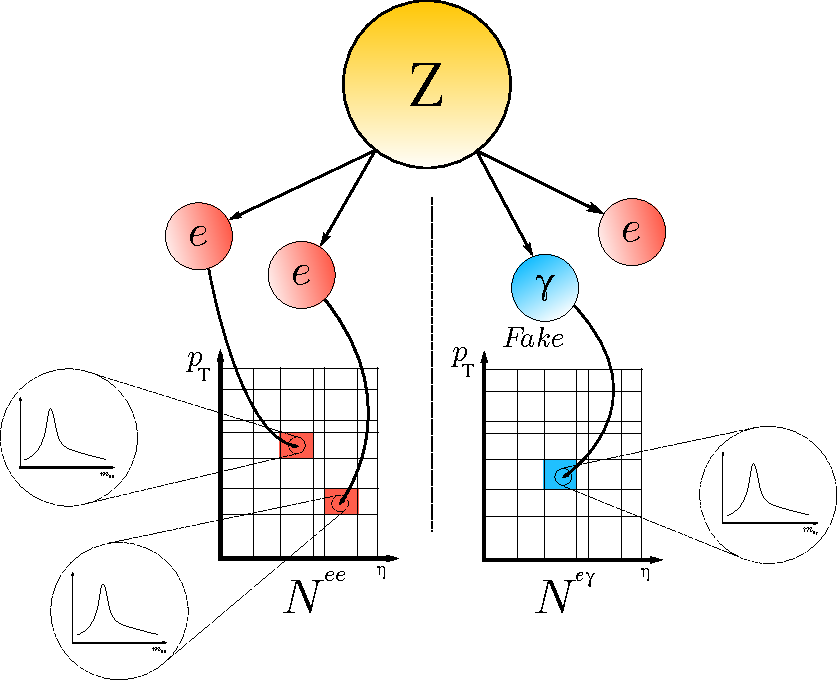
\includegraphics[width=0.6\textwidth]{images/analysis/grid_en_2.pdf}
  \caption{Esquema de reconstrucción de las distintas distribuciones de masa invariante utilizadas en el método. Cabe destacar que la clasificación en \pt de la imagen se heredó de un método anterior, pero actualmente solo se utiliza la clasificación en $|\eta|$. Si bien la imagen parece favorecer el número de pares de $ee$, en realidad es porque se está considerando tanto al electrón leading como al sub-leading, cosa que ocurre de forma similar para los pares $e\gamma$ pero no está explícito en la imagen.}
  \label{fig:efakes_matrix}
\end{figure}

Una vez ajustada cada distribución, la función se integra alrededor del pico del $Z$ en una ventana definida como $[\mu - 3\sigma, \mu + 3\sigma]$, para obtener el número de eventos que se emplea en los factores de la Ecuación \ref{eq:efake_ff} para cada intervalo de $|\eta|$. En la Figura \ref{fig:efakes_fit} se puede observar el resultado del ajuste para la distribución de masa invariante de pares $ee$ y $e\gamma$ con $|\eta| \in [0-0.6]$. Cabe mencionar que anteriormente el método empleada una clasificación adicional en \pt, y que eso introducía un sesgo en las distribuciones que era contemplado agregando una función Gaussiana adicional, centrada en valores \tosolve{donde?}. Como actualmente se aplica un corte en $\pt>145\ \gev$ el efecto del mismo es completamente despreciable para los eventos cerca del pico del $Z$.

\begin{figure*}[ht!]
  \centering
  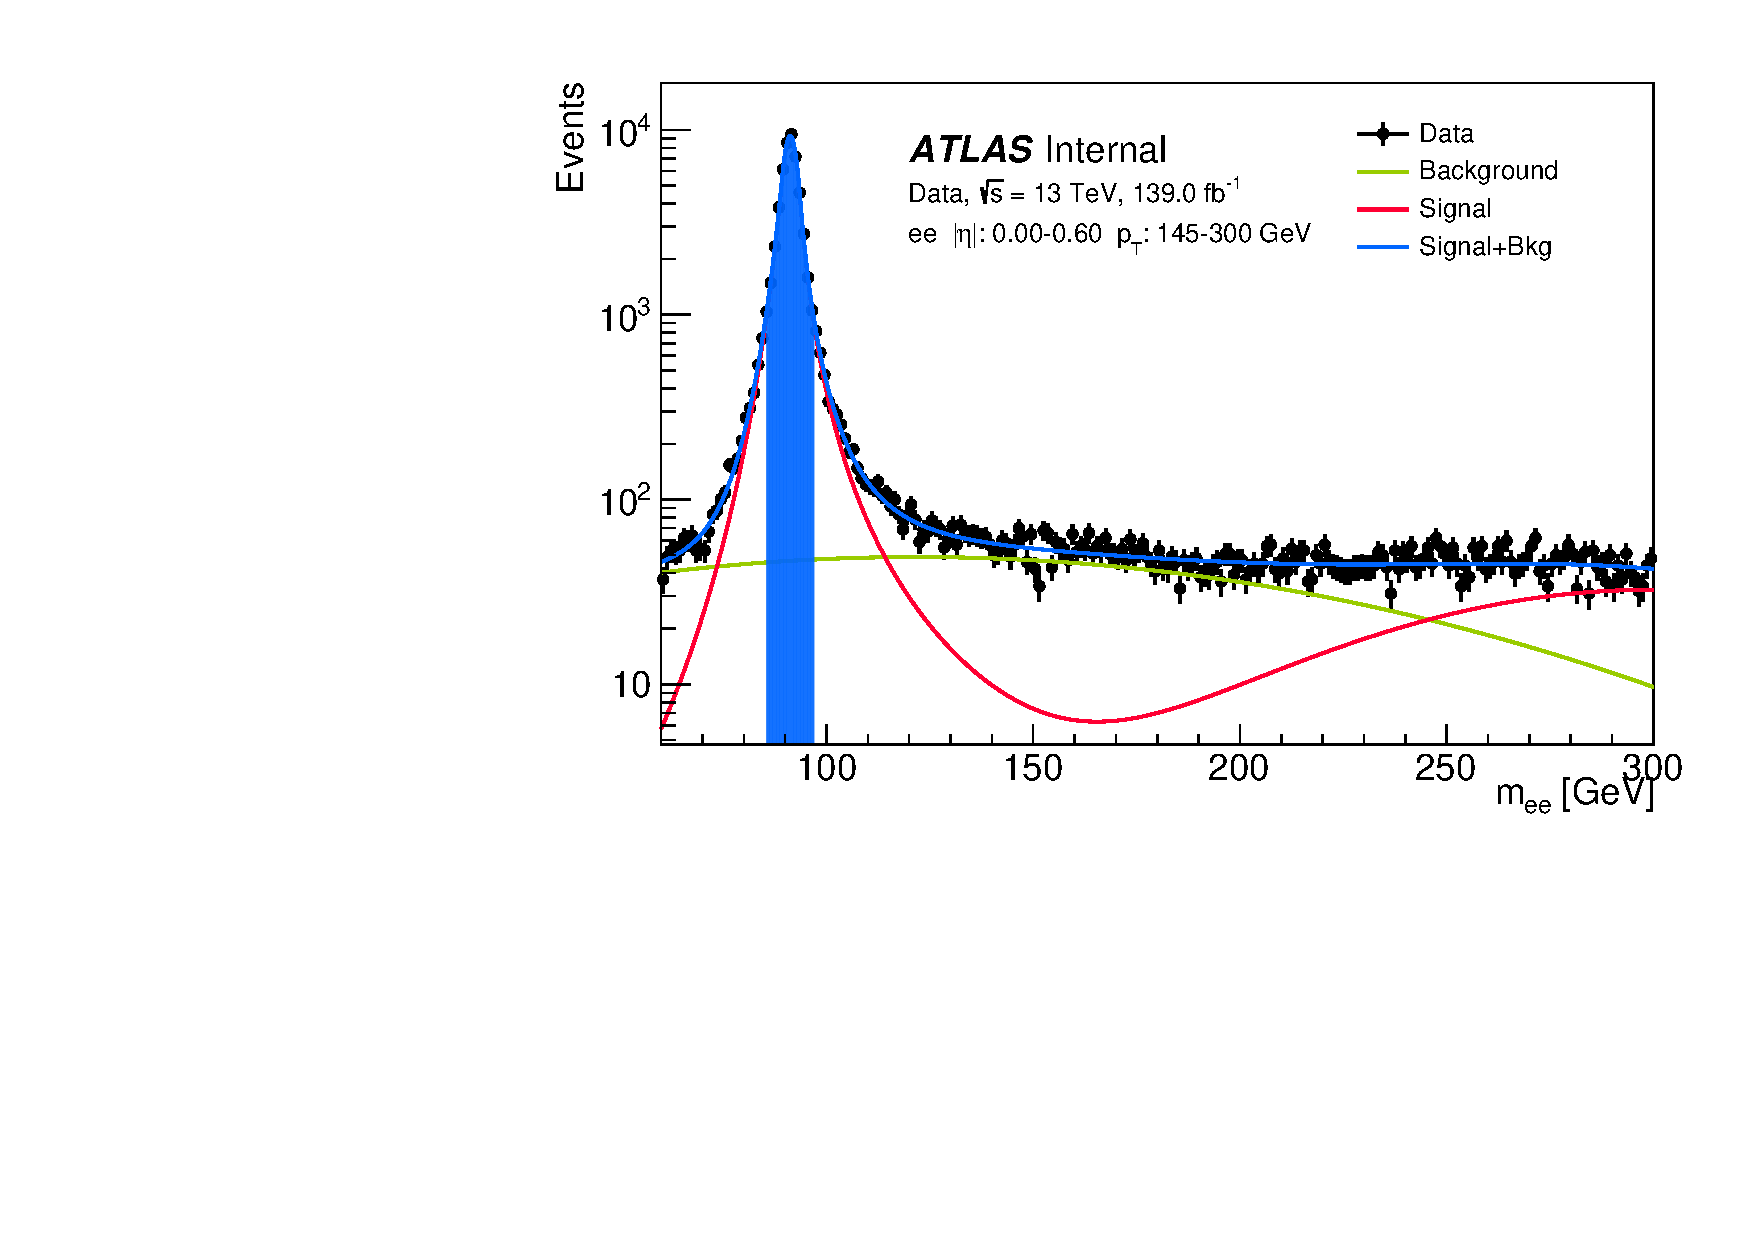
\includegraphics[width=0.45\textwidth]{images/analysis/egFF_fit_ee_eta_0_06.pdf}
  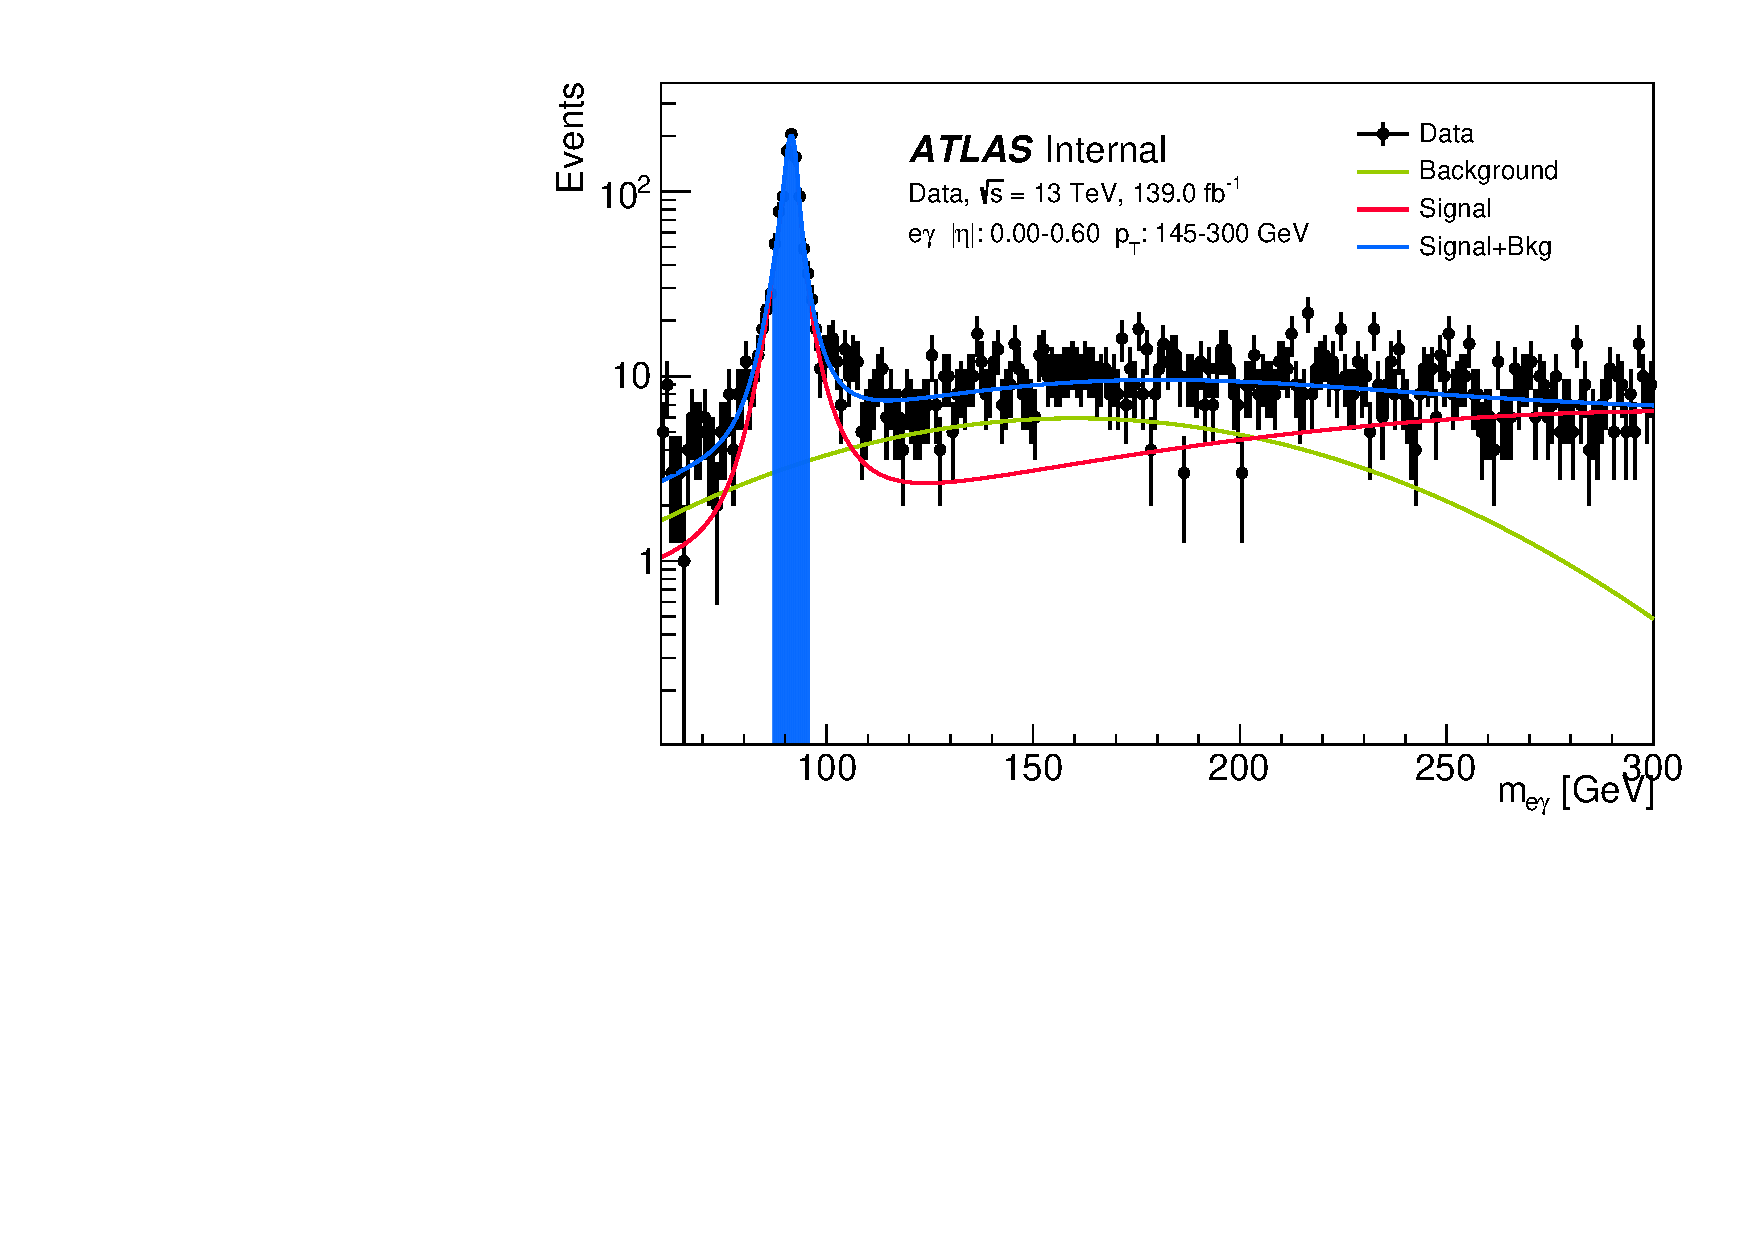
\includegraphics[width=0.45\textwidth]{images/analysis/egFF_fit_eg_eta_0_06.pdf}
  \caption{Ajuste a la masa invariante para los pares $ee$ (izquierda) and $e\gamma$ (derecha) con $|\eta| \in [0-0.6]$. La región celeste representa la ventana de integración empleada para calcular los FFs. A alto \pt una Gaussiana adicional es incluida para tener en cuenta el sesgo al aplicar un corte en \pt, pero resulta despreciable su contribución en el número de eventos cerca del pico del $Z$.}
  \label{fig:efakes_fit}
\end{figure*}

Distintas fuentes de incertidumbre sistemática fueron consideradas en el método. Se emplearon distintas ventanas de integración como $[\mu - 2\sigma, \mu + 2\sigma]$ y $[\mu - 4\sigma, \mu + 4\sigma]$. A su vez se calcularon los FFs utilizando sin la sustracción del fondo, incluyendo esta variación como sistemático que contempla el sesgo en la elección de la función de ajuste. Finalmente, como la energía del fotón `falso' es reconstruida con algoritmos para fotones, cuando en realidad deberían haber sido empleados los de electrones, se considera esto como una incertidumbre sistemática. Para ellos se calcula nuevamente los FFs ahora modificando el valor de energía de los fotones en un factor 1.5\%. Dicho valor se obtiene de las desviaciones que existen en el $\mu$ con respecto al valor de $m_Z$ de la función ajustada a los pares $e\gamma$ \cite{ATL-COM-PHYS-2016-1626}. Los valores obtenidos para los FFs junto con sus incertidumbres se pueden observar en la Tabla \ref{tab:efakes_ff}. Se puede ver como los mismos aumentan con $|\eta|$, relacionados con la cantidad de material que atraviesan y con la mayor fracción de reconstrucción de fotones convertidos con una sola traza.

\begin{table}
\centering
\caption{Factores de reconstrucción errónea de electrones como fotones en función de $|\eta|$ para todos los datos del Run 2. Se ponen explícitas las incertidumbres estadísticas y sistemáticas provenientes de variar la ventana de integración, no emplear la sustracción de fondo y el sesgo en la energía de los fotones.}
\resizebox{\textwidth}{!}{
\begin{tabular}{ l | c | c c c c | c }
\hline
\hline
\multirow{2}{*}{$|\eta|$} & \multirow{2}{*}{Fake factor} & Incertidumbre & \multicolumn{3}{c |}{Incertidumbre sistemática} & Incertidumbre \\
\cline{4-6}
 & & estadística. & V. integración & Sin sustracción & Sesgo energía & Total\\
\hline
\hline
0.00-0.60 & 0.0194 & 0.0000 & 0.0001 & 0.0006 & 0.0012 & 0.0013 \\
0.60-1.37 & 0.0244 & 0.0000 & 0.0003 & 0.0014 & 0.0001 & 0.0014 \\
1.52-1.82 & 0.0497 & 0.0001 & 0.0000 & 0.0009 & 0.0028 & 0.0029 \\
1.82-2.37 & 0.0863 & 0.0001 & 0.0007 & 0.0016 & 0.0051 & 0.0054 \\
\hline
\hline
\end{tabular}
}
\label{tab:efakes_ff}
\end{table}


Finalmente, el fondo para cada región (R) del análisis se estima definiendo una correspondiente región de control de electrones (CSE), definida de igual forma que R pero reemplazando los cortes sobre fotones por electrones. Se estima la contribución del fondo entonces como:

\begin{equation}
  N^{\text{R}}_{e\rightarrow\gamma}(|\eta|) = \text{FF}_{e\gamma}(|\eta|)\cdot N^{\text{R}}_{\mathrm{CSE}}(|\eta|)
\end{equation}

En el caso de no observar eventos en alguna CSE, se hace una estimación conservadora con un evento\tosolve{no sabia esto!!!}.

\tosolve{esto tambien se hace para jfakes, por que nunca lo hacemos explicito?}


\section{Selección de eventos y objetos para el análisis}\label{sec:selection}

El presente análisis hace uso de la totalidad de datos con una energía de centro de masa de $13$ TeV tomados con el detector ATLAS durante el Run 2 y que son aptos para física \tosolve{definir esto}, acumulando una luminosidad integrada de $139\ \ifb$. Los datos fueron seleccionados a partir del trigger \texttt{HLT\_g140\_loose}, que selecciona eventos con al menos un fotón con identificación \texttt{Loose} y con $\ET>140\ \gev$. Este trigger es completamente eficiente \cite{TRIG-2018-05}, superando el 99\% de eficiencia para $\ET>145\ \gev$, estable frente a pileup y sin dependencia con $\eta$.

Los datos y simulaciones de MC empleados para el análisis fueron preseleccionados con la derivación \texttt{SUSY1} descripta en la Sección \ref{sec:lhc_samples}, orientada a análisis con moderada actividad hadrónica y con la presencia de un fotón energético entre otras cosas.

Los objetos de interés para esta Tesis son los fotones, jets y leptones (electrones y muones) a los que se les aplica diferentes requisitos offline. Inicialmente se les requiere una selección base (\textit{baseline}) siguiendo algunas de las recomendaciones que hace el grupo de SUSY de la colaboración ATLAS y que se describe a continuación. La misma se emplea para aplicar un requisito de solapamiento (\textit{overlap removal}) entre los distintos objetos del evento y posteriormente empleados para el cálculo de \met. Finalmente a los fotones, jets y leptones se les aplica una selección denominada \textit{signal}, siendo estos objetos los que definen las distintas regiones del análisis.

\tosolve{como son cortos, capaz los siguientes items podrían ser subsubsection}

\subsection{Fotones}

Los fotones baseline deben pasar la selección de identificación \texttt{Tight}, tener $\ET>25\ \gev$, $|\eta|<2.37$ excluyendo la región del crack. Para los fotones signal se requiere adicionalmente tener $\ET>50\ \gev$, aunque para la selección de las regiones se pide adicionalmente que el fotón leading tenga $\ET>145\ \gev$ para garantizar la eficiencia del trigger. Adicionalmente se les aplica un requisito de aislamiento tanto calorimétrico como de traza, mediante el WP \texttt{FixedCutTight}.


\subsection{Electrones}

Los electrones baseline son requeridos tener $\pt>10\ \gev$, $|\eta|<2.47$ excluyendo la región crack y ser originados en el vértice primario. El requerimiento de identificación \texttt{LooseAndBLayerLLH} es aplicado \tosolve{definir o poner solo loose}. Los electrones signal son seleccionados además con $\pt>25\ \gev$, aplicando la identificación \texttt{TightLLH} y el requisito de aislamiento \texttt{FCLoose}, o \texttt{FCHighPtCaloOnly} si tienen $\pt>200\ \gev$.


\subsection{Muon}

Los muones baseline son seleccionados con la identificación \texttt{Medium}, tener $\pt>10\ \gev$, $|\eta|<2.7$ y ser originados del vértice primario. A los muones signal se les requiere adicionalmente tener $\pt>25\ \gev$ y el WP de aislamiento \texttt{Loose\_VarRad}.


\subsection{Jets}

Jets baseline son seleccionados con $\pt>20\ \gev$ y $|\eta|<2.8$. Este último requisito no es empleado en el cálculo de \met. Selecciones basadas en las trazas son aplicadas para rechazar jets con $\pt<120\ \gev$ y $|\eta|<2.4$ que se originen de las interacciones de pileup. Jets signal son seleccionados con $\pt>30\ \gev$ y $|\eta|<2.5$. La identificación de $b$-jets es empleada en la definición de algunas regiones de control. Para ello se utiliza el algoritmo \texttt{MV2c10}, con una eficiencia de selección de los mismos del 77\%.

\subsection{Overlap removal}

Como se mencionó en capítulos anteriores, los algoritmos de reconstrucción pueden fallar en los criterios de ambigüedad entre objetos, decidiendo almacenar simultáneamente a ambos. Una forma de lidiar con esto es eliminando al objeto que comparta alguna región espacial del detector con otro, en lo que se denomina overlap removal \cite{Adams:1743654}. Esta eliminación se hace en diferentes pasos, y en cada uno hay un objeto eliminado en presencia de otro. Los objetos eliminados en un dado paso no influye en los sucesivos.
El overlap removal sigue unas recomendaciones diseñadas específicamente para el tipo de análisis \cite{ATL-COM-PHYS-2016-1518}, y los diferentes pasos aplicados en el presente análisis se resumen a continuación: 

\begin{itemize}
  \item los muones CT que compartan traza con algún electrón de se eliminan
  \item los electrones que compartan traza con algún muon se eliminan
  \item los fotones que tengan $\Delta R<0.4$ con algún electrón se eliminan
  \item los fotones que tengan $\Delta R<0.4$ con algún muón se eliminan
  \item los jets que tengan $\Delta R<0.2$ con algún electrón se eliminan
  \item los electrones que tengan $\Delta R<0.4$ con algún jet se eliminan
  \item los jets con número de trazas menor a 3 y que tengan $\Delta R<0.2$ con algún muón se eliminan
  \item los muones que tengan $\Delta R<0.4$ con algún jet se eliminan
  \item los jets que tengan $\Delta R<0.4$ con algún fotón se eliminan
\end{itemize}


\subsection{Energía transversa faltante}

El cálculo de \met se realiza de acuerdo a lo descripto en la Sección \ref{sec:met}. Los depósitos de energía en el calorímetro son asociados a los objetos de alto \pt en el siguiente orden: electrones, fotones, jets y muones. Las trazas que no fueron asociadas con ninguno de los objetos anteriores son incluidas en el término soft. Para el análisis una vez hecha la selección final de los objetos se hace una selección de eventos con $\met>50\ \gev$ \tosolve{chequear}.


\section{Definición de las regiones del análisis}

Una vez obtenidas las muestras de señal y una primera estimación de los fondos del SM, el objetivo del análisis es poder diseñar regiones de señal que permitan hacer una discriminación entre ambos. Este proceso se denomina optimización y fue descripto en la Sección \ref{sec:optimization}. El mismo consiste en obtener del espacio de parámetros, la combinación de requisitos (cortes) que maximice la significancia (Ecuación \ref{Agregar}). La optimización se realiza en primer instancia conociendo a priori la cinemática del estado final del fondo y señal, y luego mediante un proceso iterativo para encontrar los valores de cortes más óptimos. Si bien el objetivo es maximizar la significancia se intenta no tener regiones muy dependientes del modelo. Con el objetivo de evitar problemas extremos de estadística o con el manejo de sistemáticos, se buscaron regiones que no tengan un número de eventos de fondo nulo, poniéndose un mínimo requerido de tres eventos. 

Una vez definidas las SRs, se puede proceder a la definición de las regiones de control y validación. Estas determinan un paso clave en el análisis para poder lograr un correcto modelado de los fondos del análisis. Las CRs se diseñaron para encontrar la normalización de los fondos principales del análisis mediante un ajuste de solo fondo a los datos. Las VRs en cambio fueron diseñadas cubriendo el espacio de parámetros entre las SRs y las CRs, con el objetivo de verificar que el modelado de los fondos es correcto. Como ambas hacen uso de los datos es indispensable que las mismas sean ortogonales a las SR para evitar un posible sesgo en los resultados finales.

A continuación se detallan los pasos que se siguieron en la optimización hasta el diseño final de las SRs y sus respectivas CRs y VRs.

\subsection{Selección de eventos de señal}

El estado final del modelo bajo estudio consiste en al menos un fotón, presencia de jets y elevada \met, como describe el diagrama de la Figura \ref{fig:phb_feyn}. Para seleccionar eventos con al menos un fotón es necesario el trigger de fotones simple con menor umbral y sin prescale, el cual es el \texttt{HLT\_g140\_loose}, por lo que a todos los fotones leading de las regiones se les solicita tener $\pt>145\ \gev$, donde el trigger es completamente eficiente. Una selección inclusiva en el número de fotones contempla el caso en el que ambos \ninoone decaen mediante fotones. El decaimiento a \gravino produce grandes cantidades de \met, que se espera que sea al menos mayor a $200\ \gev$, un valor bastante más alto que los procesos usuales del SM. Los jets del estado final pueden provenir tanto de los decaimientos de los \chinoonepm o \ninotwo, como de la ISR o del decaimiento del higgs. Para el primero de los casos el número de jets va a depender de la diferencia de masas entre el gluino y el \ninoone. Si la diferencia es pequeña (escenario comprimido) el decaimiento del gluino va a ir en mayor proporción al \ninoone, por lo que la cadena será corta y el número de jets bajo. En cambio si la diferencia es grande, el gluino tiene otros gauginos intermedios para decaer hasta el \ninoone, por lo que lo hará más en múltiples etapas dejando un número de jets mayor. A su vez esta diferencia afecta al \pt del fotón y a \met. En el escenario comprimido, la masa del neutralino es relativamente alta y por ende el producto de sus decaimientos pueden ser más energéticos. A diferencia del caso con masas de neutralino bajas, donde se esperan fotones de menor \pt y menor \met. Estas diferencias entre los distintos puntos de señal motivó al diseño de tres regiones de señal, optimizadas para distintas puntos de señal. La SRH, optimizada para el escenario comprimida, caracterizada por fotones y \met energéticos, pero bajo número de jets. En contraposición, está la SRL optimizada para masas de \ninoone baja, y caracterizada por un mayor número de jets, pero con fotones y \met no tan energéticos. Finalmente la SRM fue optimizada para un región intermedia y con características de las anteriores SRs. La Figura \ref{fig:sr_design} \tosolve{agregar} muestra el espacio de puntos para los cuales fue diseñada cada SR. Finalmente, si bien se pueden generar leptones en el estado final, se aplica un veto a los mismos para evitar el solapamiento con otro análisis que realiza una búsqueda similar con fotones y leptones en el estado final \cite{diph_8TeV}.

Definidas las selecciones básicas caracterizadas por el estado final del modelo, se procede a agregar variables que hagan efectiva la discriminación de fondo y señal. Para reducir fondos donde \met es principalmente instrumental, se aplica una separación angular entre la misma y los objetos presentes en el evento. En la señal \met proviene principalmente de los \gravino, que se espera que no tenga ninguna correlación angular con los fotones y jets, a diferencia de \met instrumental que se espera que esté alineada con los mismos. En procesos donde \met proviene de la reconstrucción errónea de alguno de los objetos, es esperable que la misma esté alineada con ese objeto. Por ese motivo se aplica un corte inferior en las siguientes variables:

\begin{equation}
  \begin{split}
  \dphigammet & = \phi^{\text{leading}\: \gamma} - \phi^{\text{miss}} \\
  \dphijetmet & = \text{min}(\phi^{\text{leading}\: \text{jet}} - \phi^{\text{miss}}, \phi^{\text{sub-leading}\: \text{jet}} - \phi^{\text{miss}}) \\
  \end{split}
\end{equation}
% 
donde las diferencias se definen de tal forma de que resulten siempre entre $0$ y $\pi$.

Otra variable que se encontró de gran utilidad para la discriminación de fondo es $\HT$, la cual se define como:

\begin{equation}
  \HT = \ptph + \sum_{i \in \text{jets}} p_{\text{T}}^{(i)}
\end{equation}

Para a señal de SUSY que tiene un fotón energético con presencia de varios jets que también pueden ser energéticos, se pueden esperar valores de \HT superiores a $1500\ \gev$.

Finalmente, se empleó una variable realizaba una reducción de fondo adicional:

\begin{equation}
  R_{\text{T}}^{N} = \frac{\sum_{i=1}^{N} p_{\text{T}}^{(\text{jet}_i)}}{\sum_{i \in \text{jets}} p_{\text{T}}^{(i)}}
\end{equation}

donde $1\le N \le N_{\text{jets}}$, que representa la fracción de \pt de los primeros $N$ jets con respecto a la totalidad de jets. Para el presente análisis se encontró que la variable \rtf daba los valores más óptimos de significancia. Las señales de SUSY se espera que contengan eventos con múltiples jets energéticos y por ende valores bajos de \rtf, a diferencia de los procesos del SM con baja actividad hadrónica y de baja energía, con valores de \rtf cercanos a la unidad. Cabe destacar que esta variable sólo es posible usarla en regiones que soliciten al menos cuatro jets.

\tosolve{mencionar lo que paso con el analisis phb? que se pensaba que los bjets del higgs podian llegar a servir para una nueva SR pero la imposibildiad de reconstruirlos correctamente no presentaba ninguna ventaja con estas SR, que en definitiva ya eran sensibles al analisis}

La definición formal de las regiones de señales se muestra en la Tabla \ref{tab:sr_def}.

\begin{table}[ht!]
  \centering
  \caption{Definición de las regiones de señal SRL, SRM y SRH}
  \begin{tabular}{l|r|r|r}
    \hline
    \hline
      &        SRL    &       SRM     &         SRH \\
      \hline
      \hline
      $N_{\text{fotones}}$  & $\ge1$ & $\ge1$ & $\ge1$ \\
      \ptph&  $>145\ \gev$ &  $>300\ \gev$ &  $>400\ \gev$ \\
      $N_{\text{leptones}}$ & 0 & 0 & 0 \\
      \njet&       $\ge 5$ &       $\ge 5$ &       $\ge 3$ \\
      \dphijetmet &        $>0.4$ &        $>0.4$ &        $>0.4$ \\
      \dphigammet &        $>0.4$ &        $>0.4$ &        $>0.4$ \\
      \met&  $>250\ \gev$ &  $>300\ \gev$ &  $>600\ \gev$ \\
      \HT& $>2000\ \gev$ & $>1600\ \gev$ & $>1600\ \gev$ \\
      \rtf &       $<0.90$ &       $<0.90$ &             - \\
      \hline
      \hline
    \end{tabular}
  \label{tab:sr_def}
\end{table}




\subsection{Regiones de control y validación}

En el presente análisis se consideraron que los procesos \phj, \wph y \ttbarph eran los de mayor impacto por lo que se diseñaron regiones de control dedicadas a los mismos, denominadas CRQ, CRW y CRT respectivamente. Todas las CRs requieren al menos un fotón con $\pt>145\ \gev$ y luego un conjunto de cortes que no solo generen una buena estadística del fondo a modelar, sino también garanticen la ortogonalidad con las SRs. El corte en \HT en general es reducido con respecto a las SRs para aumentar así la estadística de los fondos, y por la misma razón el corte en \rtf se omite en todas ellas. Cabe destacar que las tres regiones de control fueron empleadas para todas las regiones de señal, a diferencia de otros análisis donde hacen uso de CRs dedicadas además para cada SR.

La producción de pares de top, en su decaimiento leptónico, genera un estado final con dos $b$-jets, dos leptones y \met. La CRT dedicada a este proceso requiere entonces la presencia de al menos dos $b$-jets y un leptón, garantizando así la ortogonalidad con las SRs. Para evitar contaminación de señal se pone un corte superior en \met, ya que la misma en este proceso se espera que no sea tan alta como en la señal de SUSY. 

La CRW dedicada a \wph se diseña de forma similar a la CRT, pero aplicando un veto en los $b$-jets para evitar una contaminación del fondo de \ttbarph.

En los procesos como \phj, donde \met es principalmente instrumental, se espera que el vector \met esté alineado con alguno de los jets. La CRQ aplica un corte superior en \dphijetmet para incrementar la abundancia de este fondo, garantizando también la ortogonalidad con las SRs. Si bien \met es baja para este proceso, se aplica un corte inferior en la misma ya que hay suficiente estadística y para no estar muy alejada de las SRs.

En la Tabla \ref{tab:cr_def} se muestra la definición completa de las tres regiones de control. \tosolve{mostrar signal contamination?}.


\begin{table}[ht!]
  \centering
  \caption{Definición de las regiones de control de control CRQ, CRW y CRT, dedicadas a los fondos \phj, \wph y \ttbarph respectivamente. En color están los cortes que garantizan la ortogonalidad con las SRs.}
  \begin{tabular}{l|r|r|r}
    \hline
    \hline
    &   CRQ    & CRW &    CRT  \\
    \hline
    \hline
    $N_{\text{fotones}}$ &   $\ge1$    &     $\ge1$ &    $\ge1$            \\
    \ptph &  $>145\ \gev$      & $>145\ \gev$ & $>145\ \gev$                  \\
    $N_{\text{leptones}}$ &   0  & \cellcolor{lightgreen} {$\ge1$}     & \cellcolor{lightgreen} {$\ge1$} \\
    \njet     &   $\ge3$   &     $\ge1$ &    $\ge2$ \\
    \nbjet   &  -   &   $0$ &   $\ge 2$ \\
    \dphijetmet  & \cellcolor{lightgreen} {$<0.4$} &     $>0.4$ &    $>0.4$ \\
    \dphigammet   &    $>0.4$   &   - &        - \\
    \met &  $>100\ \gev$  & \cellcolor{lightgreen} {$[100,200]\ {\gev}$} & \cellcolor{lightgreen} {$[50,200]\ {\gev}$} \\
    \HT &  $>1600\ \gev$ &  $>400\ \gev$  &  $>400\ \gev$      \\
    \hline
    \hline
  \end{tabular}
  \label{tab:cr_def}
\end{table}



A continuación se definen las VRs, las cuales fueron diseñadas para verificar el correcto modelado de los fondos. Las mismas se encuentran en una región intermedia entre las CRs y las SRs, siempre siendo ortogonales a estas últimas. Se diseñaron un conjunto de VRs orientadas al modelado de los fondos de \wph y \ttbarph, y otras para el de \phj. Nuevamente se requiere en todas ellas al menos un fotón con $\pt>145\ \gev$.

Se definieron cinco VRs orientadas al fondo de \phj. Estas regiones recuperan el corte en \dphijetmet de las SRs, pero agregan un corte superior en \met de $200\ \gev$, siendo así ortogonales a ellas. Entre ellas se encuentran las VRM1L y VRM1H, orientadas a validar las regiones SRL y SRH respectivamente, emulando sus cortes en \pt del fotón y \met. A su vez la VRM1L incluye un corte similar en \rtf para validar la aplicación del mismo en las SRs. Ambas tienen un corte inferior en \met de $100\ \gev$, y se desprenden de ambas regiones de validación equivalente pero con un corte inferior en \met de $150\ \gev$, denominadas VRM2L y VRM2H. Finalmente se encuentra la VRQ, que es un compromiso entre las regiones anteriores, solicitando una baja cantidad de jets y a su vez bajo \pt de fotones. La definición completa de las VRs dedicadas al fondo de \phj se muestra en la Tabla \ref{tab:vrm_def}.


\begin{table}[ht!]
  \centering
  \caption{Definición de las regiones de validación VRQ, VRM1L, VRM2L, VRM1H y VRM2H, empleadas para la validación del fondo de \phj. En color están los cortes que garantizan la ortogonalidad con las SRs.}
  %% \resizebox{\textwidth}{!}{
    \begin{tabular}{l|r|r|r|r|r}
    \hline
    \hline
    &   VRQ & VRM1L & VRM2L & VRM1H & VRM2H \\
    \hline
    \hline
    $N_{\text{fotones}}$ & $\ge1$ & $\ge1$  & $\ge1$  & $\ge1$  & $\ge1$\\
    $\pt^{\text{leading}-\gamma}$ & $>145\ \gev$ & $>145\ \gev$  & $>145\ \gev$  & $>300\ \gev$ & $>300\ \gev$           \\
    $N_{\text{leptones}}$ &  0 & 0 & 0 & 0 & 0 \\
    \njet & $\ge3$  & $\ge5$  & $\ge5$ & $\ge3$ & $\ge3$ \\
    \dphijetmet & $>0.4$ & $>0.4$ & $>0.4$ & $>0.4$ & $>0.4$ \\
    \dphigammet &  $>0.4$ & $>0.4$ & $>0.4$ & $>0.4$ & $>0.4$ \\
    \met &  \cellcolor{lightgreen} $[100,200]$ &  \cellcolor{lightgreen} $[100,200]$ &  \cellcolor{lightgreen} $[150,200]$ & \cellcolor{lightgreen} $[100,200]$ & \cellcolor{lightgreen} $[150,200]$ \\
    \HT & $>1600$ & $>1600$  & $>1600$ & $>1600$  & $>1600$\\
    \rtf &  -  &  $<0.90$ &  $<0.90$ & - & - \\
    \hline
    \hline
    \end{tabular}
    % }
    \label{tab:vrm_def}
\end{table}


Para los fondos \wph y \ttbarph se definieron cuatro regiones de validación, por lo que todas requieren al menos un leptón y lo que las hace ortogonales a las SRs. La VRL1 y VRL2 estudian la región de bajo \met y validando distintos valores de \HT, mientras que las VRL3 y VRL4 lo hacen para $\met>200\ \gev$. Además VRL4 invierte el corte en \dphijetmet para validar esa variable en regiones con combinaciones distintas de la misma. La Tabla \ref{tab:vrl_def} muestras las definiciones completas de las VRs dedicadas a estos fondos.

\begin{table}[ht!]
  \centering
  \caption{Definición de las regiones de validación VRL1, VRL2, VRL3 y VRL4, empleadas para la validación de los fondos de \wph y \ttbarph. En color están los cortes que garantizan la ortogonalidad con las SRs.}
  \begin{tabular}{l|r|r|r|r|r}
  \hline
  \hline
   & VRL1 & VRL2 & VRL3  &  VRL4     \\
  \hline
  \hline
  $N_{\text{fotones}}$  &  $\ge1$ &   $\ge1$  &    $\ge1$   &  $\ge1$     \\
  $\pt^{\text{leading}-\gamma}$   &   $>145\ \gev$  &  $>145\ \gev$   & $>145\ \gev$  &  $>145\ \gev$  \\
  $N_{\text{leptones}}$   & \cellcolor{lightgreen}{$\ge1$}  & \cellcolor{lightgreen}{$\ge1$} & \cellcolor{lightgreen}{$\ge1$}  & \cellcolor{lightgreen}{$\ge1$}  \\
  \njet   &   $\ge2$ &  $\ge2$  & $\ge2$   &   $\ge2$     \\
  \dphijetmet & $>0.4$  &  $>0.4$  & $>0.4$   & \cellcolor{lightgreen}{$<0.4$}  \\
  \met & \cellcolor{lightgreen}{$[50,200]\ \gev$} & \cellcolor{lightgreen}{$[50,200]\ \gev$} &  $>200\ \gev$  &   $>200\ \gev$     \\
  \HT &  $>800\ \gev$ &  $>1300\ \gev$   & \cellcolor{lightgreen}{$[600,1600]\ \gev$} &  $>1100\ \gev$  \\
  \hline
  \hline
  \end{tabular}
  \label{tab:vrl_def}
\end{table}

